\documentclass[11pt,a4paper]{article}
\usepackage[margin=25mm]{geometry}
\usepackage{amsmath,amssymb,booktabs,graphicx,array}
\usepackage[section]{placeins}
\usepackage[font=small,labelfont=bf]{caption}
\PassOptionsToPackage{hyphens}{url}
\usepackage[colorlinks=true,urlcolor=blue,citecolor=blue]{hyperref}
\setlength{\parskip}{0.4em}
\setlength{\emergencystretch}{3em}
\makeatletter\setlength{\@fptop}{0pt}\makeatother
\title{Experience-dependent behaviour and material persistence in cellular bodies}
\author{Cellular Automata Research Project\\Research in progress; authorship under discussion}
\date{20 October 2026}
\usepackage{longtable}
\begin{document}
\maketitle
\begin{abstract}
Learning in artificial life requires experience to alter a continuing body's useful responses, yet acquired state, responsive physiology and material renewal can produce similar outward behaviour. We address this ambiguity with a comparative experimental framework that specifies the information available to a learner, intervenes on acquired content at matched bodily states and measures the resulting physical costs. Across distinct cellular models, local scalar consequences establish an action direction without a supplied reward gradient; controlled cue encounters support preference reversal and reassignment of temporal credit; and conditional experience changes the allocation of protective reserves. These effects have different limits. Scalar response estimation acquires in both tested conditions but reverses reward preference in only one, while a fixed responsive control also succeeds after an execution change. In a regenerative host, acquisition coincides with substantial tissue production, but newborn-content interventions do not establish that copying learned values is necessary for subsequent behaviour. At equal protection purchases, acquired conditional readout reduces injury by 16.6\% and 5.1\% relative to pooled content in two parents; its advantage over immediate physiology depends on environmental stability and contact timing. Together, the experiments distinguish useful acquired content from capabilities supplied by sensing, actuation and physiology. They establish conditional physical functions of experience, while leaving a unified, continuously adapting and regenerating learner unresolved.

\end{abstract}
\section*{Introduction}
Artificial-life systems can grow, move and preserve organized structures through local interactions. A further challenge is to make a continuing body learn from the consequences of its own actions. This requires more than an interesting trajectory: experience must change internal content, that content must contribute to subsequent behaviour, and the body must remain able to obtain and use new evidence. When material also flows, consumes energy and disappears, learning and physical persistence become coupled experimental questions.

Continuous cellular automata make these questions concrete. Lenia and its extensions produce localized and interacting structures, while parameter search discovers sensorimotor behaviours\cite{chan,expandedlenia,plantec,hamon,asal}. Neural cellular automata support growth and regeneration\cite{growingca,developmental,bricks}. Runtime plasticity, meta-learning and differentiable updates provide routes towards adaptation during operation\cite{khajehabdollahi,pdnca,duan,wang,miconi,backpropamine}. These achievements do not, by themselves, distinguish a rule selected by an external optimizer from content acquired within an individual's lifetime. Nor does a history-dependent response establish an advantage over an equally informed fixed physiological rule.

The distinction is especially important when information is supplied by the experimental interface. A controller receiving a reward gradient already knows a useful direction. A system observing completed displacements can estimate an execution map unavailable to a scalar-outcome learner. A recent-feedback rule may solve a delayed association task if no competing event intervenes. Conversely, a learner can fail because its own behaviour prevents contact with new evidence. Evaluating endpoints without specifying these interfaces confounds acquired capability with the observations and actions installed in advance.

Studies of non-neural organisms motivate treating memory as a physical process rather than assigning it from appearance alone. Habituation, environmental traces, network reorganization and retained responses can all connect past conditions to future behaviour\cite{boisseau,reid,kramar2021,vogel,boussard,reiber}. Regulatory and collective dynamics offer further forms of persistence\cite{acar,micheelsen,yang,lambert}. Transporting a state with tissue, however, does not establish that its content is learned or necessary. Regeneration adds a separate requirement: behavioural use must persist when its original material carrier is actually lost\cite{shomrat}.

Here we organize these distinctions into three experimental tests. First, we specify what the learner can observe and compare it with simple rules using the same lawful information. Second, we branch complete acquired bodies and manipulate only the proposed content, retaining physical state and randomness at the branch. Third, we measure the resulting movement, energy, injury and tissue production. Strong controls and physical accounting are essential because learning can be costly and its benefit depends on environmental timing\cite{mery2005,dunlap2009,mitchell,tagkopoulos}. Matched branches test mechanisms within histories; they do not create additional independent learning histories.

We apply this framework to three explicitly separated implementations: conservative moving bodies for action and cue learning, resource-constrained generative bodies for admission and persistence, and an externally supplied density-regulated birth/death model for behaviour during tissue production and predictive maintenance. The main results proceed from scalar action acquisition to controlled temporal credit, then to spatial consequences and conditional physical utility. Seven figures connect behavioural tests, actual fields and resource accounts. Standard learning rules serve as experimental instruments; the contribution is the resolved relationship between acquired content and physical outcomes, rather than a claim to a new general optimizer. The models jointly identify requirements for a regenerating learner, but their separate positive results are not combined into evidence that one such learner has already been achieved.

\section*{Results}
\subsection*{Local paid consequences can establish an action direction without a supplied gradient}

Our primary action-learning test restricts the learner to consequences that its own moving material actually receives. A conservative, deformable cellular body starts with no learned response direction on a periodic $32\times32$ domain. Its local policies can read transported internal records, a locally completed scalar energy gain or loss, a receipt that motion was paid, and their own exploration randomness. The actual transport operator $K$ moves material and these records but supplies no displacement observation to the learner. Neither reward gradients, coordinates, the external field, the physical actuator rotation nor an environmental change flag enter the policy. This restriction separates the present capability from interfaces that supply a gradient or a completed displacement (Fig.~\ref{fig:scalar-action}).

Movement axes, cohesion, pressure, energy transduction, exploration and material transport remain engineered capabilities. Two noise seeds are paired with opposite unknown actuator rotations, while the initial reward meaning is the same. These are two constructed conditions, not independent draws from a population of environments. Actual outcomes are available throughout a dense finite substrate. The task tests whether these local scalar experiences can establish useful action in an unfamiliar execution relationship; it does not test sparse encounter recovery, discovery of a sensor, or learning during tissue birth.

We compare standard accumulated action updates, the same updates with scalar state features, a fixed run-and-tumble response and a random policy. A subsequent prospectively fixed single-trajectory perturbation-response estimator maintains a moving estimate of the correlation between its action perturbation and the change in its actual scalar outcome over a completed eight-step action block. Its normalized estimate sets the next mean command. It receives no additional observation and has the same action bound and exploration schedule. The estimator and its normalized readout change together, so the comparison does not isolate an advantage of the estimator alone. The method is a standard local response rule, rather than a new optimizer or a measurement of the body's exact mechanical Jacobian.

Both response-estimation lives pass acquisition. Their final-64-step mass-weighted field scores are $0.63550$ and $0.63274$. After an unannounced reversal of reward meaning, the corresponding scores are $0.14684$ and $0.27984$: only the second condition passes the original complete phase criterion. In the subsequent 128 steps without new payments, outcome observations or parameter writes, both pass, with scores $0.53410$ and $0.60963$. These aftereffects do not repair the first condition's failed reversal. The first body's first continuous 32-step favourable interval occurs at step 678, after the reversal interval ended at 640; the second reaches that measure at 628. Neither result is recovery after a single new feedback event.

The strong comparisons constrain the interpretation. Both accumulated-action and scalar-context updates acquire in both conditions but pass neither reversal nor the aftereffect. Adding the tested state features therefore supplies no additional capability. Fixed run-and-tumble acquires in one condition and random action in neither; neither passes the later phases. The complete five-method, two-condition, three-phase results and all phase costs remain in the accompanying source-data tables. The response-estimation bodies finish at energies $121.308$ and $124.319$, spending $2.56720$ and $2.57260$ on movement. Fixed run-and-tumble spends less, $2.10862$ and $2.16194$, while finishing at $119.388$ and $119.294$. Useful acquired behaviour need not minimize movement expenditure, but the expenditure is part of its physical consequence.

\subsection*{Acquired direction contributes to an aftereffect without explaining every retained success}

We next branch each complete response-estimation body at step 640, including the body that failed its reversal window. Clearing its response estimate or rotating it by $90^\circ$ is followed by 128 actual steps without new feedback or writes. Original retained-content tails are reused as recorded references, not simulated again. Density, energy, other internal records, physical coupling, random state and clock agree at branching; the intervention changes only the declared response content. Rotation preserves each local estimate's norm, although the componentwise actuator nonlinearity means it need not preserve actual commands or costs.

Retained, cleared and rotated estimates produce aftereffect scores $0.53410/0.22435/0.14044$ in the first parent and $0.60963/0.34531/0.19537$ in the second. Both retained futures pass, one cleared future passes, and neither rotated future passes. Direction content therefore changes the physical future, while the acquired body's position and continued motion also contribute to occupancy. Clearing does not freeze the body: random commands, material transport and physical costs continue. The surviving cleared success rules out attributing every aftereffect to the retained direction. The two parents and their related futures are mechanism comparisons, not six independent acquisitions (the accompanying source-data tables).

\subsection*{Execution changes require responsiveness, but a fixed response rule can suffice}

Changing reward meaning and changing the action--consequence relationship pose different problems. From the two actual response-estimation parents at step 320, we retain the original reward meaning and change only the hidden physical execution rotation. Each parent supplies continued estimation, frozen estimation and fixed run-and-tumble futures. The last control is explicitly endowed with the same acquired initial direction. It can use subsequent scalar outcome changes and the same random innovations, but does not fit a response vector. It is a strong acquired-state control, not an independent life-zero acquisition.

Over the final 64 steps of the 320-step paid continuation, continued estimation scores $0.88986/0.86846$, frozen estimation $-0.23287/-0.29387$, and fixed run-and-tumble $0.71258/0.70763$. The corresponding no-new-feedback scores are $0.85625/0.76574$, $-0.25315/-0.28661$ and $0.71991/0.72083$. Continued estimation and the fixed response both pass in both parents; frozen estimates pass neither. The fixed response also spends less on motion: $1.20366/1.21010$ versus $1.42209/1.38288$ for continued estimation. Higher scores in the latter do not establish a unique algorithmic capability from two related parents, different response forms and different realized expenditure (the accompanying source-data tables).

All these futures start in a favourable region. An early passing residence interval consequently cannot identify rapid relearning; the late departure of frozen futures and sustained outcomes under both responsive policies provide the relevant comparison. The experiment establishes finite action learning from local paid scalar experience and a role for its acquired direction. It also shows that a simple fixed response to new outcomes can maintain useful behaviour after an execution change. Ten new life-zero trajectories and ten actual parent continuations constitute twenty recorded paths, not twenty independent repetitions. All retain approximately mass 24 in this series, with no tissue birth. Their positive outcomes cannot be combined with regeneration in a different host to claim one continuously learning, renewing organism.

\begin{figure}[p]
\centering
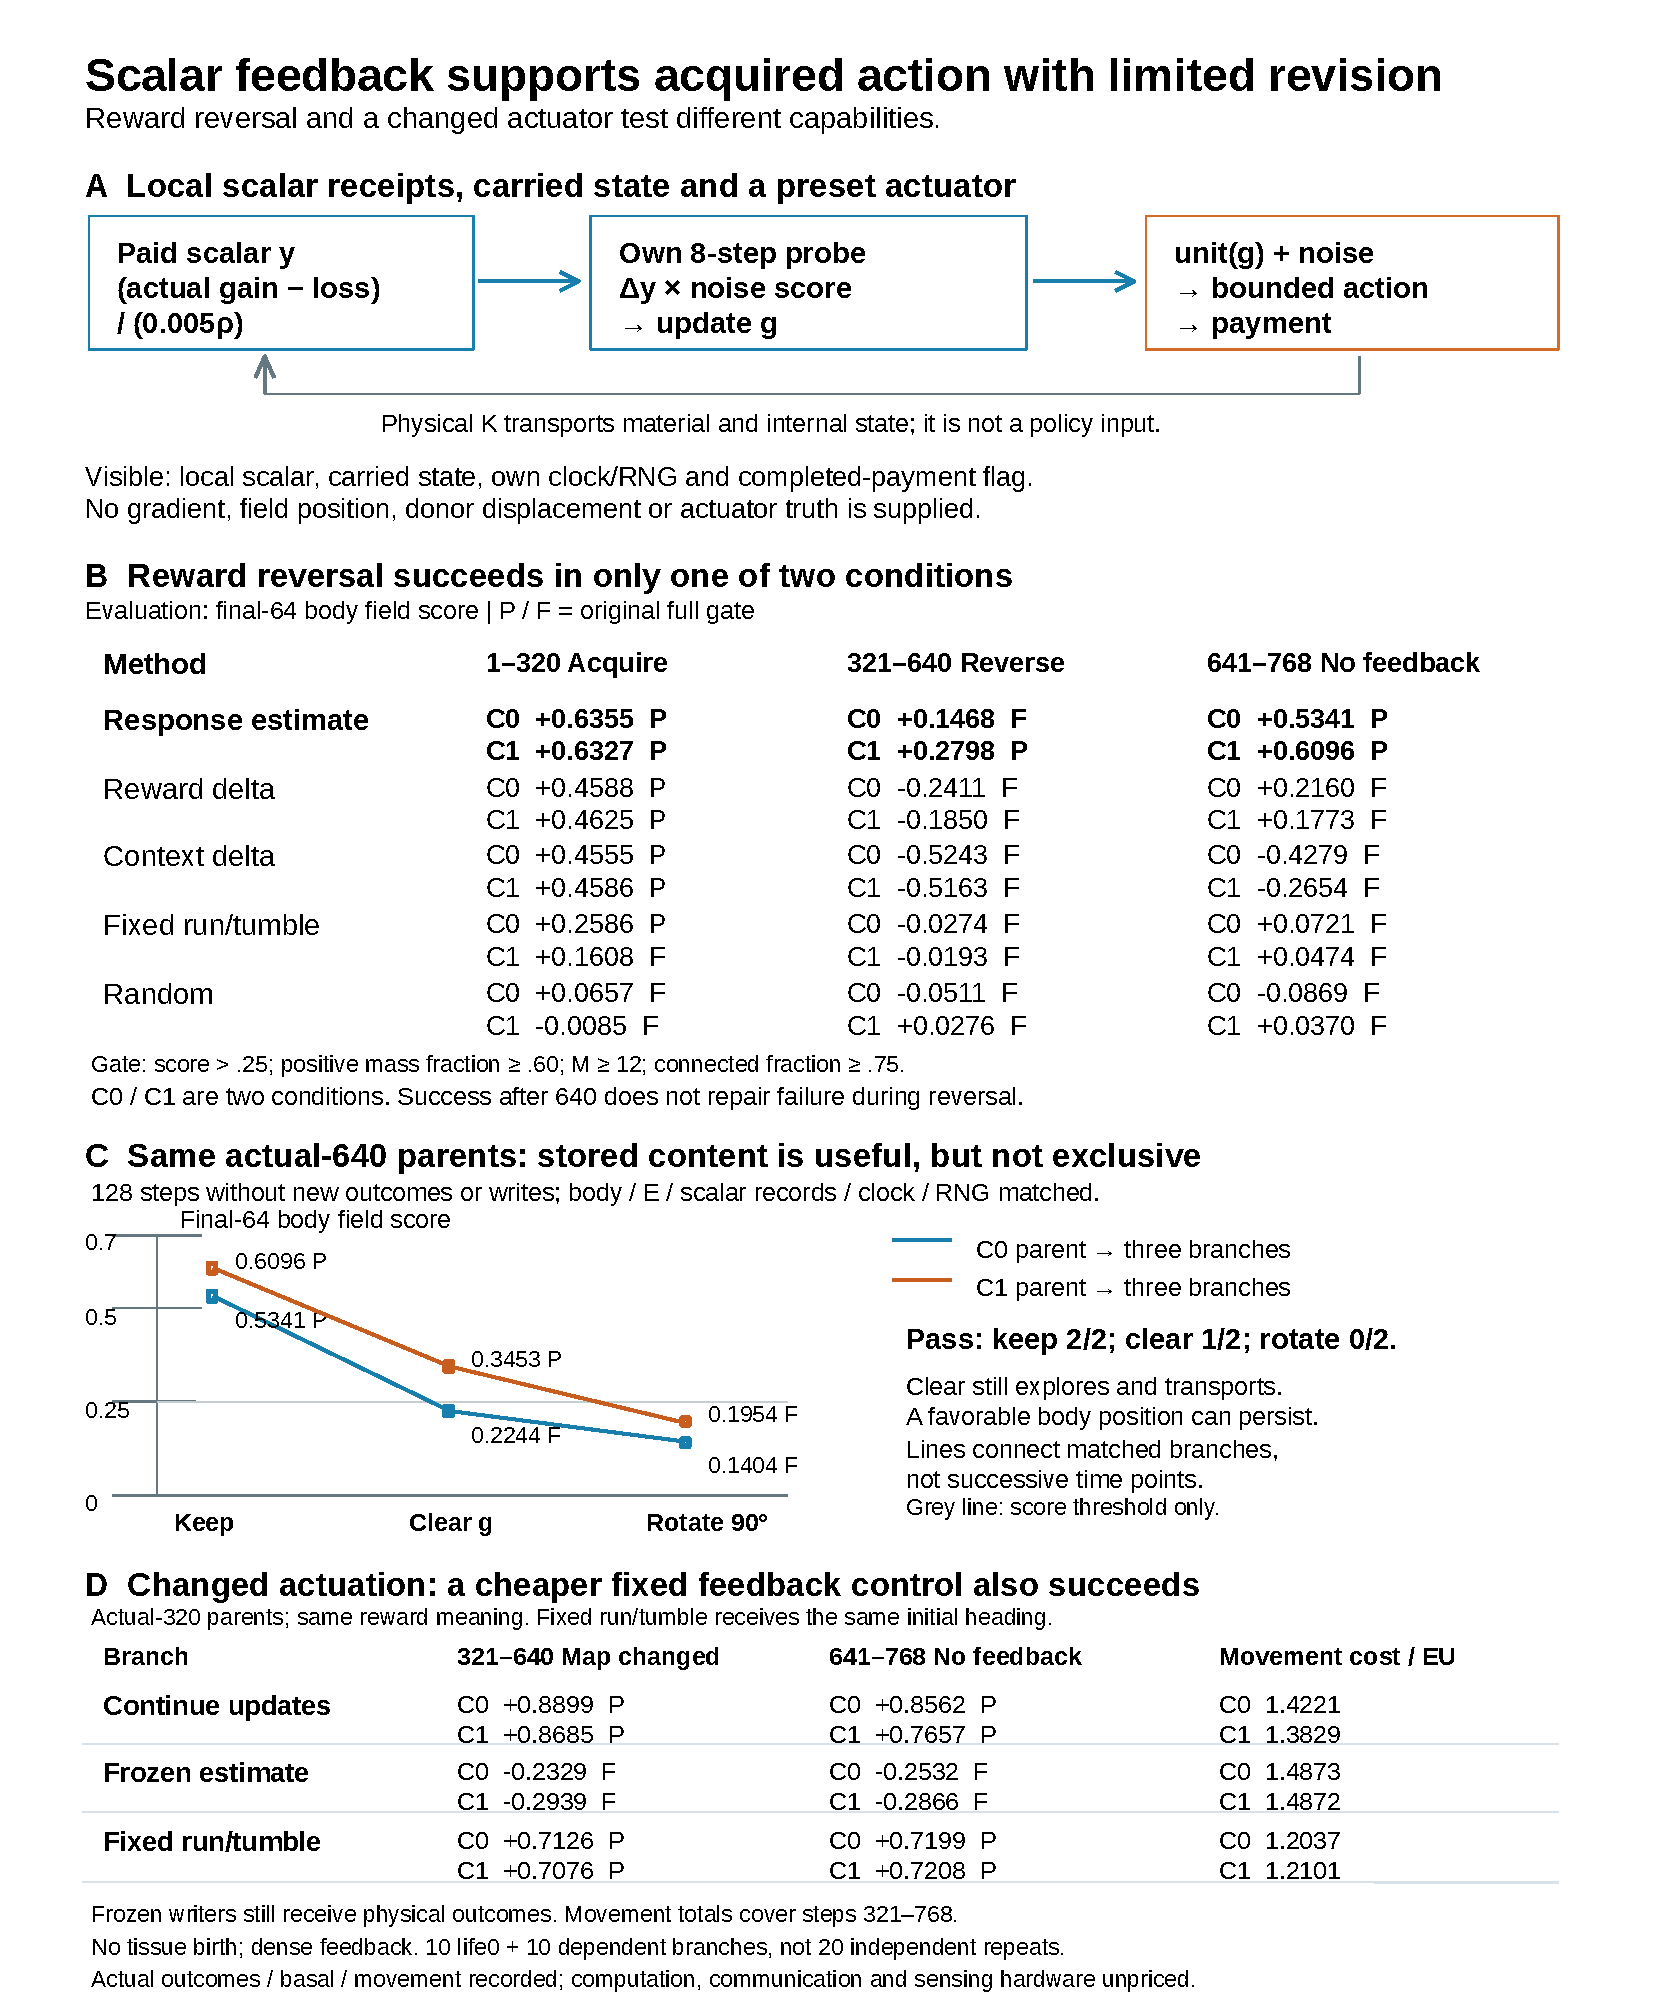
\includegraphics[width=\linewidth,height=0.68\textheight,keepaspectratio]{work/longform_v047/figures/scalar_action_v048/scalar_action.pdf}
\captionsetup{font=footnotesize}
\caption{\textbf{Scalar-only experience supports action acquisition, with different limits under reward and execution changes.}
\textbf{a}, A standard local response estimate uses completed scalar outcome changes and physically carried perturbation records. The transport operator $K$ moves material and internal state but provides no learner-facing displacement, gradient, field coordinate or actuator truth. Motion axes, cohesion, exploration and energy measurement are supplied.
\textbf{b}, All five methods, two paired seed--actuator conditions and three phases. Cells give final-64 mass-weighted field scores and the original complete gate (P/F); these evaluation quantities are not policy inputs. Response estimation passes acquisition in both conditions, reward reversal in one and the following no-new-feedback interval in both. The later success does not revise the failed reversal.
\textbf{c}, Two actual step-640 parents with response retained, cleared or rotated. Lines join related content interventions, not successive times. Retention passes twice, clearing once and rotation never. Clear branches still explore and move; rotation preserves response norm but not each bounded command or expense. Retained tails reuse recorded trajectories without replay.
\textbf{d}, From actual step-320 parents, only the physical execution map changes. Continued estimation and fixed run/tumble both pass the paid and later no-new-feedback windows in both conditions; frozen estimation fails. The fixed control receives the same acquired initial heading and spends less on movement. Expenditure sums both continuation phases. Ten new life-zero paths and ten dependent branches are not twenty independent repetitions. The conservative host has no tissue birth; physical expense is reported without a separate tariff for computation or sensing hardware. All phase outcomes and accounts are retained in the accompanying scalar-action source tables.}
\label{fig:scalar-action}
\end{figure}


\subsection*{A continuing cellular body acquires and reverses a cue preference}

Controlled cue encounters isolate learning of an outcome relationship from learning how to direct an action. The assay keeps one deformable cellular body through acquisition, a neutral interval, an unannounced contingency reversal and a second neutral interval. Two cue channels are initially assigned opposite local feedback signs. After exposure, a probe presents the cues on opposite sides of the body without reinforcement. Later exposure reverses which cue predicts the positive outcome. The learner is not supplied with a phase label, the reversal time, the environmental mapping or a desired action. Its available signals are the local cues and the energy gain or loss actually delivered to tissue. An appropriate response must consequently depend on the experienced association rather than on a supplied task identifier.

The body is a continuous density and intracellular-energy field on a periodic $32\times32$ lattice. Local paid transport changes its spatial distribution; cohesion and pressure support a connected deformable organization. It is not a rigid particle following a prescribed centre trajectory. However, this implementation has no regenerative birth and does not use a trained Lenia growth rule. The sensing channels, cohesion, cue-gradient actuator and conversion of local energy feedback into a signed teaching signal are supplied components. The experiment tests whether plastic state can acquire and revise the relation between those channels and outcomes within a continuing body; it does not test the emergence of the sensors, actuator or learning rule.

Three update conditions share these bodily dynamics. A non-plastic reactor retains its initial cue values. A strong recent-feedback rule updates the value of the most recently registered cue with unit learning rate. An eligibility-trace rule updates values using a decaying local cue trace and learning rate $0.5$. Both plastic rules use a normalized prediction error based on realized local feedback. Values and their associated cue records travel with the actual tissue transport. Their use follows established ideas of associative updates and eligibility\cite{sutton,florian,izhikevich,fremaux}; implementing these ideas locally in the present body is not, by itself, an algorithmic invention.

The completed assay contains two random seeds and both orders of the initial cue--feedback mapping. These give four related seed--order conditions per arm and pairing condition. There are 24 continuing 960-step life trajectories, followed by 24 value-preserving and 24 value-erased continuations. The latter are paired forks of the same terminal bodies, not additional independent acquisition histories. All 72 paths remain alive under the specified mass and connectivity criterion. The four seed--order conditions should not be described as four independent random seeds, and the many local cue contacts are not independent biological replicates.

With paired feedback, both plastic rules show strong appropriate cue contact after acquisition (Fig.~\ref{fig:lifetime-learning}). The endpoint contact fraction at the first acquisition probe averages $0.999993$ for the recent-feedback rule and $0.999993$ for the eligibility rule, compared with approximately $0.5$ for the reactor. Following a neutral interval, the corresponding means remain $0.999967$ and $0.999996$. These fractions measure the share of actual probe contact assigned to the currently correct cue, rather than a classification score computed directly from the internal values. They therefore include the body's movement and spatial encounter with the two probe regions.

After the cue--feedback relation reverses, both plastic rules redirect contact towards the newly positive cue. Their first post-reversal probe means are $0.999994$ and $0.999986$. At the final retention probe, the recent-feedback mean is $0.989435$, with individual values from $0.978865$ to $0.999998$, and the eligibility mean is $0.999998$, with values from $0.999997$ to $0.999999$. The result establishes re-acquisition after an unannounced change within this protocol. It does not establish immediate reversal upon the environmental change, nor transfer to arbitrary cue schedules, geometries or resource regimes. The first post-reversal probe follows eight completed feedback pulses, four for each cue. No independent choice score was recorded during forced exposure, so recovery after a single feedback event is not established.

Pairing controls are essential to this interpretation. Unpaired exposures retain the cue and feedback opportunities but balance positive and negative feedback for each cue. Across opposite mapping orders their mean correct-contact fraction is approximately $0.5$. This aggregate does not mean that every unpaired body remains indifferent. Some unpaired acquisition probes show nearly exclusive contact with one cue, producing very small or very large correct-contact fractions depending on the assigned mapping. At the final reversal-retention probe, unpaired eligibility values span approximately $0.0164$ to $0.9836$. The pairing comparison therefore identifies the usefulness of experienced cue--outcome correspondence across the tested conditions; it does not equate absence of reliable correspondence with absence of an internally acquired preference.

\begin{figure}[p]
\centering
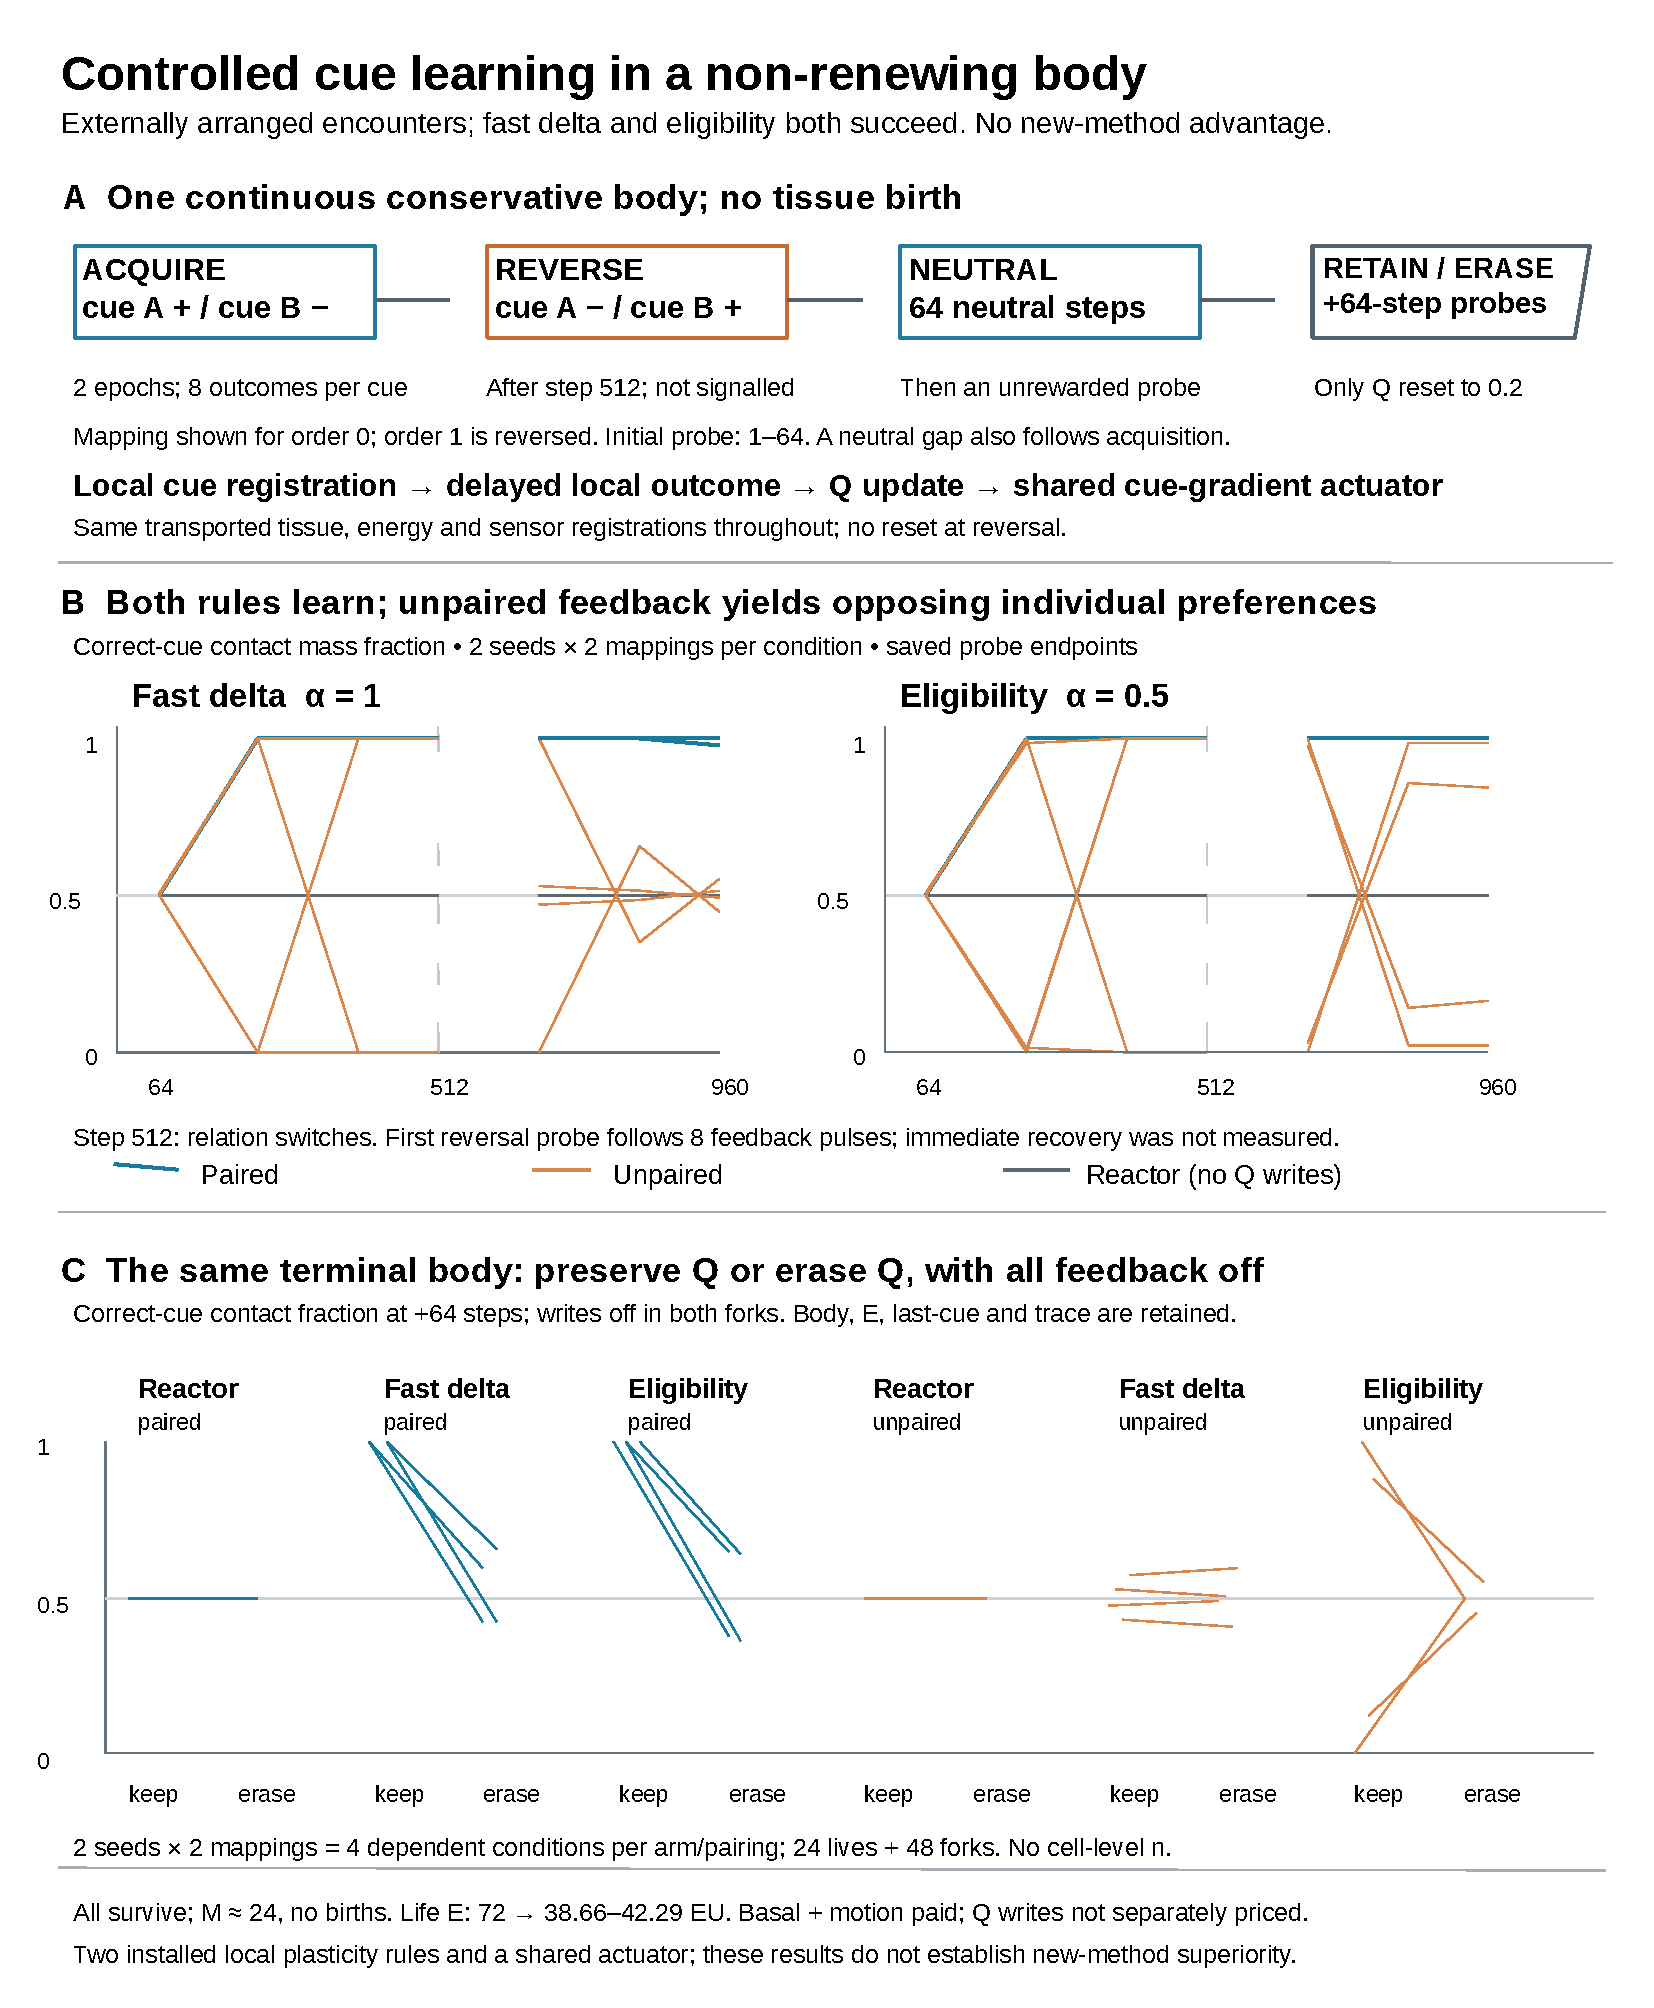
\includegraphics[width=\linewidth,height=.76\textheight,keepaspectratio]{work/longform_v047/figures/lifetime_learning_v0474/lifetime_learning.pdf}
\caption{\textbf{Controlled cue learning in a non-renewing body.}
\textbf{a}, Externally arranged encounters on one continuing conservative body, without tissue birth. \textbf{b}, Two installed update rules, recent-feedback (fast delta) and eligibility, acquire and reverse cue preference in a continuing transported body. Four related seed--mapping paths per condition retain the individual outcomes: the unpaired mean near one half hides opposing preferences. \textbf{c}, Matched terminal freeze/erase forks change only the initial stored cue values, preserving body, energy and sensory registrations at branching. The first reversal probe follows eight new feedback pulses. All paths survive in this no-birth host, while movement and basal costs reduce available energy. Neither update rule establishes a new-method advantage. Values are actual probe contact fractions; repeated phases and terminal forks are not independent histories.}
\label{fig:lifetime-learning}
\end{figure}



\subsection*{Erasure reduces preference, while successful behaviour still has a physical cost}

To test expression after acquisition, each terminal body is continued for another 64 unreinforced steps with value writing disabled. One branch retains its learned cue values, and the other resets those values to the common initial value of $0.2$. Density, energy, cue traces and the rest of the terminal bodily state are retained. This is a targeted value-erasure comparison at a shared state, rather than a replay of acquisition or a replacement of the whole body with a naive initialization.

In paired recent-feedback bodies, the value-preserving branch reaches a mean appropriate-contact fraction of $0.9999997$, whereas erasure reduces it to $0.5211$; individual erased outcomes range from $0.4194$ to $0.6533$. In paired eligibility bodies, the corresponding means are $0.9999988$ and $0.5075$, with erased outcomes from $0.3618$ to $0.6494$. The comparison supports a role for the stored values in expression during this terminal probe. Values are not the only history-dependent part of the body: erasure leaves the acquired geometry, energy distribution and other local records in place. The residual spread after erasure is thus informative, and should not be rounded into a claim of exact restoration of a pristine naive state.

The behavioural gain occurs in a body that continues to pay for movement and basal activity. Mean movement expenditure across paired 960-step lives is $3.4661$ for recent feedback and $3.3788$ for eligibility, compared with $2.1551$ for the reactor. Basal expenditure is $27.648$ in all these groups. Actual feedback gains and losses also differ because the bodies evolve differently during exposure. Mean terminal energy is $42.0836$ for paired recent feedback, $41.9749$ for paired eligibility and $42.1969$ for the paired reactor. Thus successful cue choice does not require a larger final energy reserve than the non-plastic control. A screening rule demanding simultaneous improvement in behaviour and every bodily total would reject this meaningful behavioural change for the wrong reason.

This does not remove the need for physical accounting. The result is bounded by the viability of the actual body and by the resources supplied in the protocol. Initial mass and energy are 24 and 72; no starvation or injury loss occurs in these runs, and movement payments are met. The reported energy account closes to numerical precision. However, the additional arithmetic required to update and read values is not separately assigned a physical energy cost. The assay therefore measures movement and basal costs under its specified model, rather than the complete thermodynamic cost of learning. It also provides no evidence that the body can replenish its material indefinitely: the continuing body is conservative and has no birth process.

The recent-feedback control is deliberately strong. It can retain the latest cue through the delayed feedback interval and use that record to update values rapidly. Its success means that the present delay structure does not establish an advantage of the eligibility rule. The small difference at the final retention probe is not a basis for declaring a general superiority, given two seeds, related mapping orders and highly saturated probe performance. The experiment instead supplies a usable behavioural benchmark: acquired preference, reversal and retention are observable within one continuing cellular body, while matched non-plastic, unpaired and erasure controls limit alternative explanations. Longer or conflicting delays, unfamiliar contexts and concurrent bodily replacement remain distinct questions.


\subsection*{Changing which past event predicts feedback requires temporal credit reassignment}

The success of recent feedback in the controlled cue assay leaves an important ambiguity: remembering the latest cue may suffice because no competing cue intervenes before its outcome. A second experiment separates the information in recent and earlier contact. Each lesson presents one cue, a brief gap, a statistically independent second cue and another gap before local feedback. All four earlier--recent cue combinations occur within each block. Initially the earlier cue determines the outcome. The body must therefore retain information across a distractor rather than merely respond to the last event (Fig.~\ref{fig:temporal-credit}).

Five update conditions share the physical host and visible local records. Recent-cue delta uses the latest registered event; a fixed exponential trace mixes recent experience; a fixed earlier-event delta uses the known task lag; joint delta learns four coefficients over both cue identities at both lags; and a two-expert gate adjusts the weight assigned to the two temporal sources from their local prediction errors. The fixed earlier-event control is deliberately informed about the original delay structure. Joint delta and the gate receive both records but no instruction identifying which one determines feedback. The gate is an established type of error-weighted combination, not a claim of a newly discovered learning algorithm.

Two new seeds and two initial cue-meaning orders give four conditions per rule. Fixed earlier-event delta, joint delta and the gated experts each pass all six acquisition, meaning-reversal and retention probes in all four conditions, with the continuing bodies alive. Recent-cue delta and the particular fixed trace tested here each pass the complete six-probe sequence in zero of four conditions. One recent-cue life and two fixed-trace lives fail the predefined connectivity condition; their mass remains near 24 and energy remains positive. These are losses of the required connected individual, not total material extinction. Incomplete and unobserved probes remain incomplete or missing. The negative result for this exponential trace does not establish failure of eligibility traces in general.

The harder continuation changes the predictive temporal source without changing the cue identities' positive and negative meanings. At step 1216, all seventeen surviving complete physical states continue without resetting their bodies, value banks, traces or cue registrations. The most recent event now determines feedback. Each rule inherits its own actual acquired history, so cross-rule comparisons include the different bodies and internal states produced earlier. They are not algorithm substitutions into one identical parent. The three previously failed lives remain failed and are not restarted.

Joint delta and the gate pass all three prescribed probes in all four continued conditions. The fixed earlier-event rule fails at least one probe in every condition. Its two seed-7403 paths retain the wrong preference at the final retention probe; both seed-7404 paths recover after an initial probe near $0.48$. The surviving recent-cue and fixed-trace subsets pass three of three and two of two continuations, respectively. These subset successes are expected to become possible when recent contact is now relevant, but they do not erase the earlier failures or become four-of-four success over the complete history.

\begin{figure}[p]
\centering
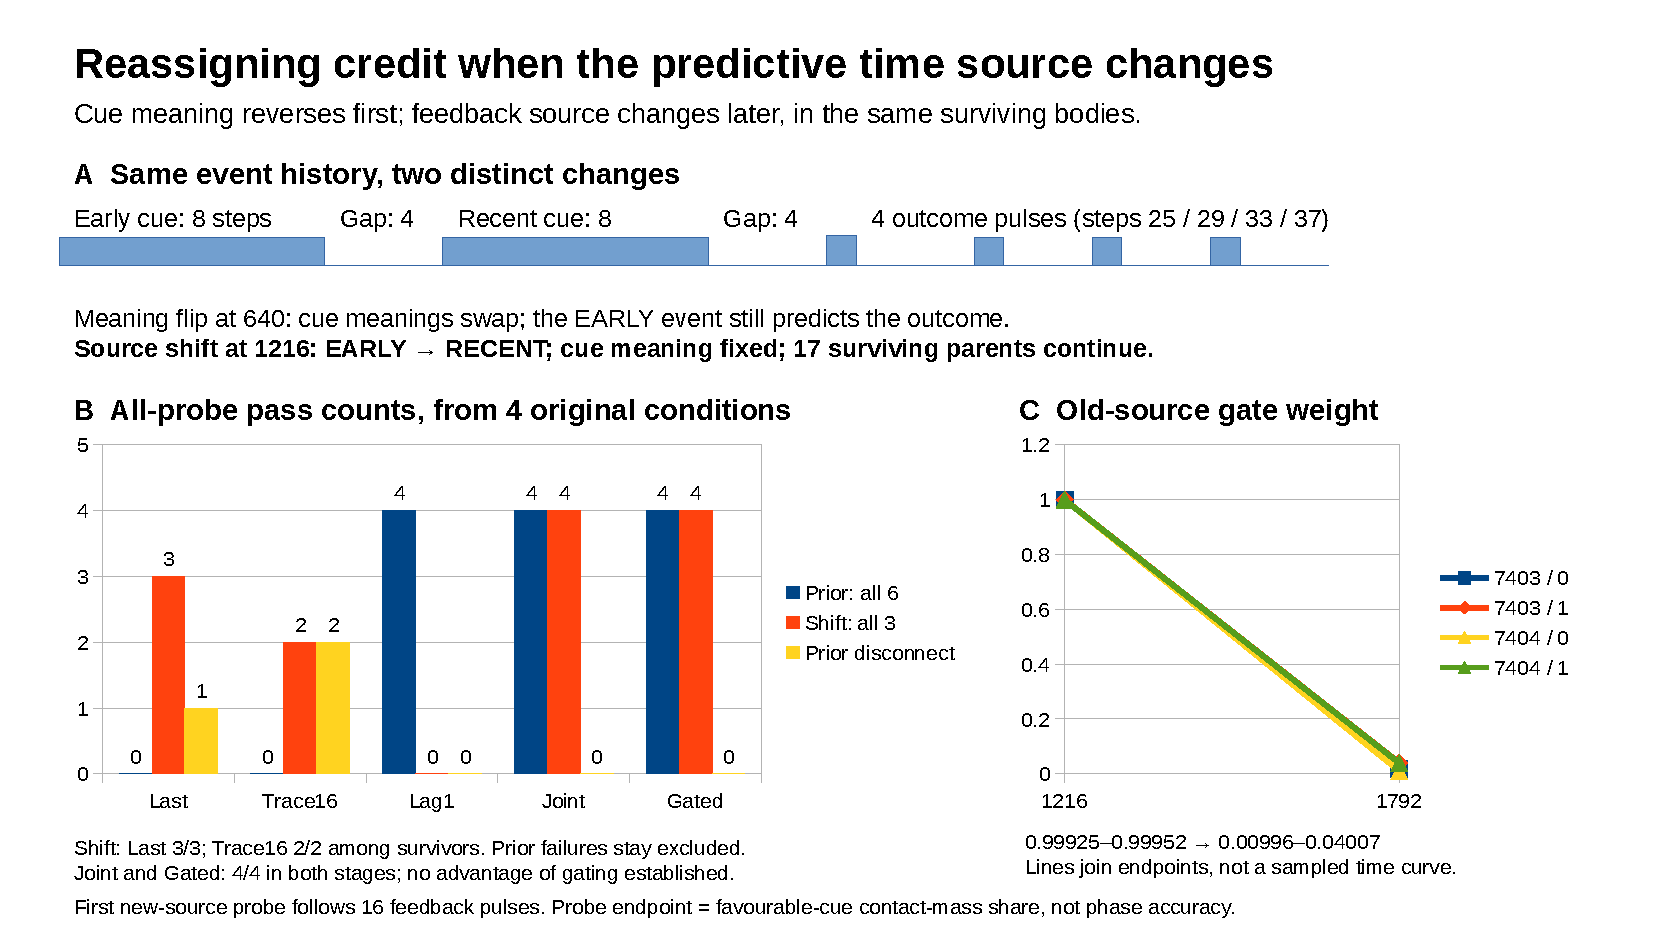
\includegraphics[width=\linewidth,height=.76\textheight,keepaspectratio]{work/longform_v047/figures/temporal_credit/temporal_credit.pdf}
\caption{\textbf{Useful history changes when the predictive temporal source changes.}
\textbf{A}, An independent intervening cue separates earlier from recent contact. The first change reverses cue meaning; the later change makes the recent event predictive while preserving cue meaning. Seventeen surviving bodies continue without reset. \textbf{B}, Fixed earlier-event delta, joint delta and gated experts pass all six initial acquisition, reversal and retention probes in four related seed--order conditions. Joint delta and gated experts also pass all three later probes in four of four conditions; fixed earlier-event delta fails a phase in all four. Earlier connectivity failures in recent-cue delta and the fixed trace remain failures. Their later three-of-three and two-of-two successes describe surviving subsets, shown relative to the original four-condition count. \textbf{C}, Individual gated-rule weights shift from the earlier to the recent source. Lines join the two measured endpoints and do not depict the intervening time course. Joint delta achieves the same behavioural coverage. Probe values are favourable-cue contact-mass fractions at the final frame; the first changed-source probe follows sixteen feedback pulses. These conservative bodies do not regenerate tissue, and additional learning arithmetic is not physically priced.}
\label{fig:temporal-credit}
\end{figure}


The gate supplies a direct internal readout of temporal reassignment. Across its four paths, the body-weighted earlier-source weight changes from $0.99925$--$0.99952$ at the boundary to $0.00996$--$0.04007$ after the changed-source continuation. This is a change between two available temporal hypotheses, driven by experienced local outcomes. Joint delta achieves the same behavioural coverage without an explicit gate, however, so successful reassignment does not establish that the gated architecture is necessary or superior. Terminal energy and movement costs also differ across paths: joint-delta energy ranges from $14.34$ to $17.83$, and gated energy from $13.91$ to $17.18$, with overlapping movement-expenditure ranges. The analysis retains these physical consequences without demanding that every cost or reserve improve for learned behaviour to count.

The measurements resolve a finite capability, not instantaneous adaptation. The first new-source feedback arrives after 24 updates without an informative new outcome. The first subsequent choice probe occurs after sixteen feedback pulses. Probe scores are the favourable-cue share of contact mass at the probe's last frame, not the proportion of correct decisions across the entire exposure stage. Following the changed relation, neutral intervals and matched value-freeze and association-erasure forks again distinguish retained expression from continued correction. Erasure reduces the learned preferences but leaves body, energy and sensory history intact; residual preferences cannot be called erasure of all memory.

These comparisons advance the behavioural question from fixed cue association to selection between past sources of evidence. They also show what has not advanced: sufficient simple joint history already solves the tested problem. The lessons and actuator remain supplied, broad training fields permit feedback at weak contact, the material host has no birth, and controller arithmetic and storage are not physically charged. Self-generated experience in a fixed arena and retention through regeneration remain open. The continuous actual animation preserves the old and changed-source segments, including the stopped histories, so the claim rests on continuing bodies rather than resetting an agent for each successful phase.







\subsection*{Writing changes spatial development without a uniform survival advantage}

We next examine why bodily expression cannot be reduced to the strength of an internal value. From one complete acquired body and its remaining environment at step 240, we compare continued local writing with stopping new writes. The stopped branch retains state decay, eligibility, transport and the remaining movement dynamics. The two futures therefore start from identical acquired physical state and differ in subsequent writing, rather than in the amount of prior experience or in a reset of all internal variables (Fig.~\ref{fig:writing-turnover}).

The actual density scenes at steps 400, 560 and 720 show progressively different spatial organizations. At 560, continued writing retains more mass, 20.72 versus 16.13. Yet 56.23\% of that mass has specific energy below $0.08$, compared with 16.85\% in the stopped branch. By 720 the mass ordering reverses: 5.90 remains with writing and 8.72 without further writing. Total energy has the opposite ordering, 4.755 versus 1.170. Over the common continuation, reduced injury loss under writing is outweighed by additional starvation loss: the continued-minus-stopped differences are $-6.062$ and $+8.889$ in the respective mass-loss accounts.

\begin{figure}[p]
\centering
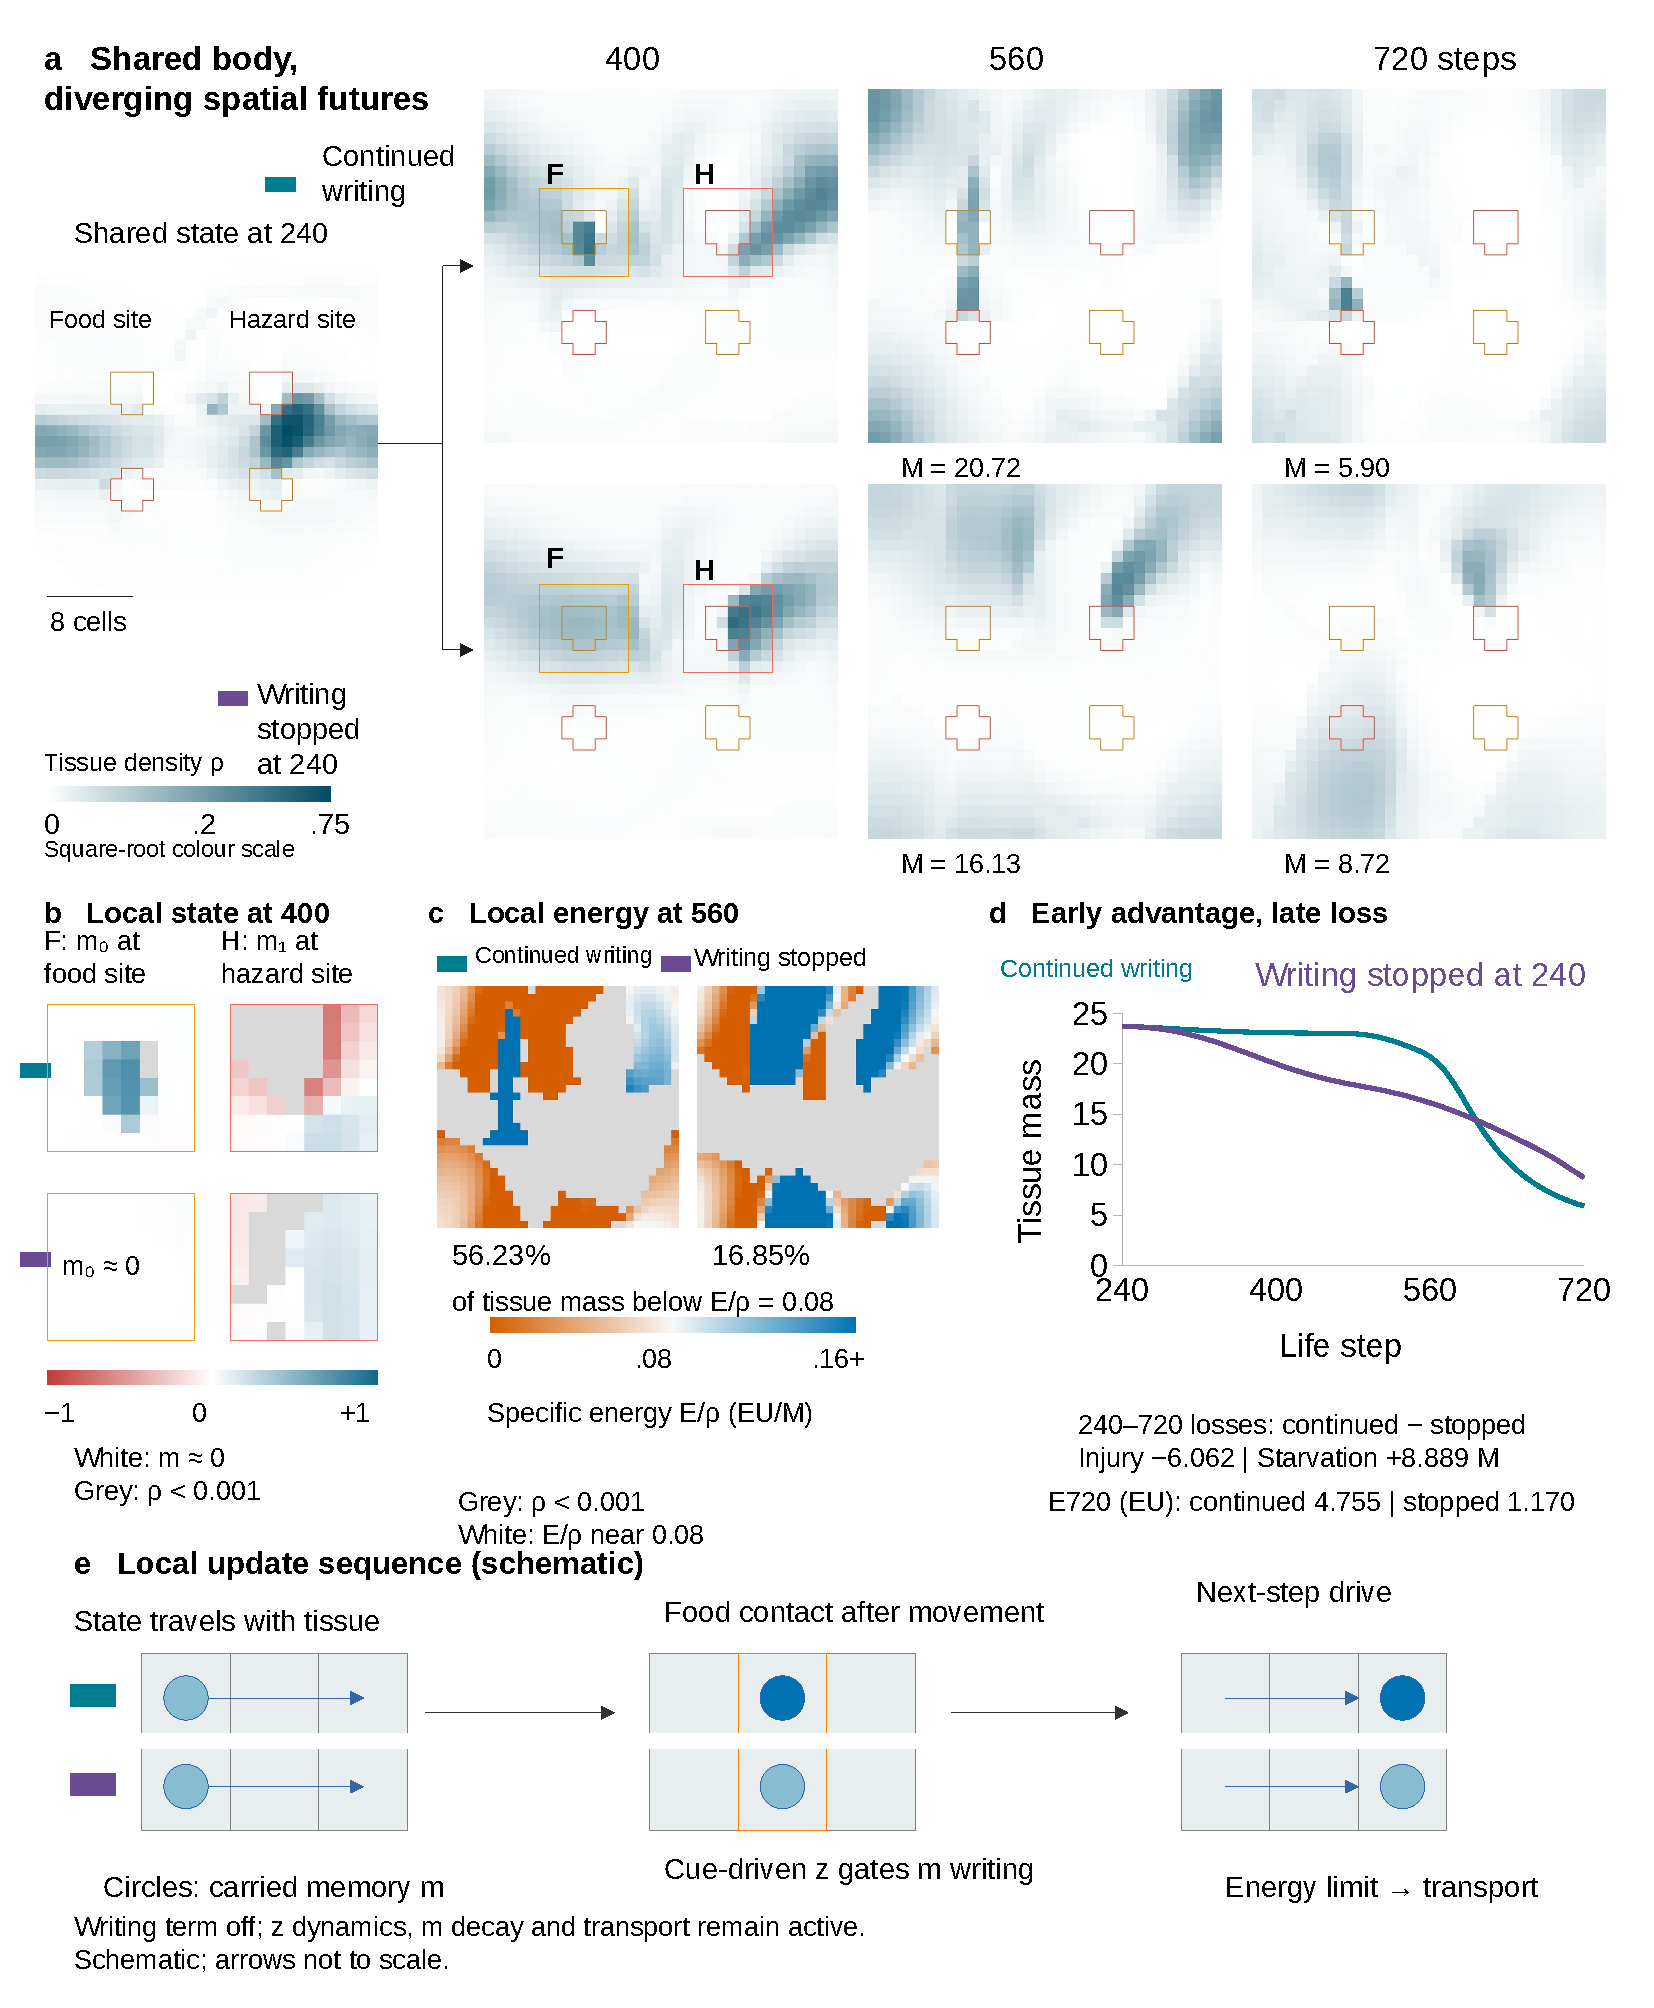
\includegraphics[width=0.90\linewidth]{figures/main/spatial_experience/spatial_state_divergence.pdf}
\caption{\textbf{Shared body, diverging spatial futures.}
\textbf{a,} The same complete acquired body and remaining world at step 240 continue with writing enabled (teal) or new writing stopped (purple). Density scenes at 400, 560 and 720 retain original periodic $32\times32$ coordinates and the same square-root colour scale. F/H mark Food/Hazard sites; F here is a food-site label, not the fuel F of Fig.~\ref{fig:allocation-feedback}. Scale bar, 8 cells.
\textbf{b,c,} Local $m_0/m_1$ at 400 and specific energy at 560 are observed fields, not isolated mediators. Grey masks $\rho<0.001$; low-energy percentages include all tissue mass.
\textbf{d,} The complete 61-point mass path shows early advantage followed by late loss; final energy has the opposite ordering.
\textbf{e,} Schematic of transport, cue-driven eligibility and writing, then subsequent energy-limited movement. Stopping new writing leaves $m$ decay, transport and eligibility active. This model has no tissue birth and is distinct from the generative models; the continued-writing future is reused.}
\label{fig:writing-turnover}
\end{figure}


These observations explain why the spatial process belongs in the main argument. An earlier mass advantage can contain a larger population of poorly fuelled tissue, and different loss mechanisms can reverse a later ordering. The local food- and hazard-associated fields and specific-energy maps reveal where those differences are expressed. They do not identify a unique mediator: local state, energy, shape and subsequent encounters change together after branching. The experiment contains one acquired history and no tissue birth, and its continued-writing future is reused from an existing trajectory. It consequently provides a resolved example of coupled physical consequences, not a population-level estimate of a general learning benefit.

This interpretation is compatible with energetic approaches to active motion\cite{schweitzer,circle,tjhung} and with the broader observation that collective movement depends on distributed interactions\cite{tonertu}. It does not require treating every changing pattern as learning. The evidence is useful because it exposes the actual route from internal-state manipulation to different local resource conditions and loss processes. A successful integrated learner must be evaluated at both levels: the behaviour elicited by experience and the physical trajectory through which that behaviour remains possible.

\subsection*{Conditional acquisition can coexist with real tissue production in a different host}

To test behaviour alongside actual tissue production, we use a distinct material CA in which local density regulates birth and death while an installed central controller reads acquired cue values. This model preserves paid material transport and local birth admission, but its generation rule is not the original Lenia kernel response. Extracellular stocks receive measured external supply. It is a reusable experimental host for behavioural questions about real tissue production and loss, rather than evidence that the earlier Lenia rule or the local non-renewing motor body has acquired these capabilities (Fig.~\ref{fig:young-turnover}).

The behavioural question also requires separating experienced consequences from direct tissue selection. In preceding injury-based tests, continuing value updates improves safe contact relative to retaining stale values, but resetting those values without further writing reproduces much of the improvement. A fixed prior can pass acquisition. These controls prevent attributing the entire difference to a newly learned useful response. The subsequent energetic task changes the local consequence: actual uptake is followed by an energy tax that enters heat rather than directly deleting tissue according to cue identity. Feedback uses completed uptake minus the amount of tax actually paid. Real physiological death, starvation, birth and transport remain possible; the condition is not a physically lossless learning model.

Two opposite meanings are applied to each of two supplied initial geometries. In the compact geometry, a standard current-feedback update acquires the favourable response in both conditions, while the matched fixed prior does not. Final-64 safe-contact fractions are $0.81632$ and $0.76208$, versus $0.58561$ and $0.60644$ with the fixed prior; absolute safe-contact masses are $75.136$ and $68.963$. At the acquired step-256 checkpoints, $83.225\%$ and $83.700\%$ of the actual body is material born after life zero. This establishes conditional acquisition alongside substantial real tissue production in that same implementation. It does not establish that copying the acquired content into new material explains the behaviour. Net growth accompanies birth and loss, so the newborn fraction is not a one-to-one fraction of founding tissue replaced.

The alternative elongated geometry provides two acquisition counterexamples. Neither compact condition passes the registered final reversal window after the outcome meaning changes, and the elongated conditions fail that reversal criterion as well. Among the later compact stop-writing endpoints, only one fast condition passes. Four elongated main paths lack their planned 128-step terminal segments after a storage stop; these missing windows remain unavailable, not zero-valued failures or successful continuations. The original same-parent future-writing controls and all fixed-prior results remain in the accompanying source-data tables. Neither opposite meanings nor initial geometries are treated as independent random replications, and the conditional acquisition is not a new-method advantage.

To test newborn content more directly, each of the two qualifying complete step-256 compact parents branches for 128 updates with new writing disabled and the acquired meaning unchanged. Actual newborn tissue receives the local pre-write copy, a zero payload under the same tariff, or a norm-preserving swap of cue contents. Surviving old content is untouched and all initial physical states and histories match. Physical uptake and energetic feedback continue: this is stop-writing expression, not no-feedback retention. Tissue born during the probe comprises $58.798\%$--$60.466\%$ of its final body. All six branches retain the registered safe-contact behaviour. In the first parent, all three physical and action histories are exactly equal despite nonzero content differences. In the second, safe fractions are $0.83241$, $0.83326$ and $0.82582$ for copy, zero and swap; action differences occur without changing the passing outcome. Thus correct newborn copying is not necessary in this tested window. It does not follow that all inherited content is irrelevant: old tissue remains and its contents are not erased.

The joint interpretation is deliberately architectural. Original Lenia generation, conservative local motor learning and this externally supplied density-regulated birth/death model answer different questions. The last now demonstrates standard conditional acquisition during tissue production, whereas the local-motor experiment demonstrates content-dependent action without birth. Neither yields the full repeated revision and maintenance of useful experience through turnover. Their costs and negative controls specify what an integrated explanation must account for, without combining separate hosts into one continuous adaptive life.

\begin{figure}[p]
\centering
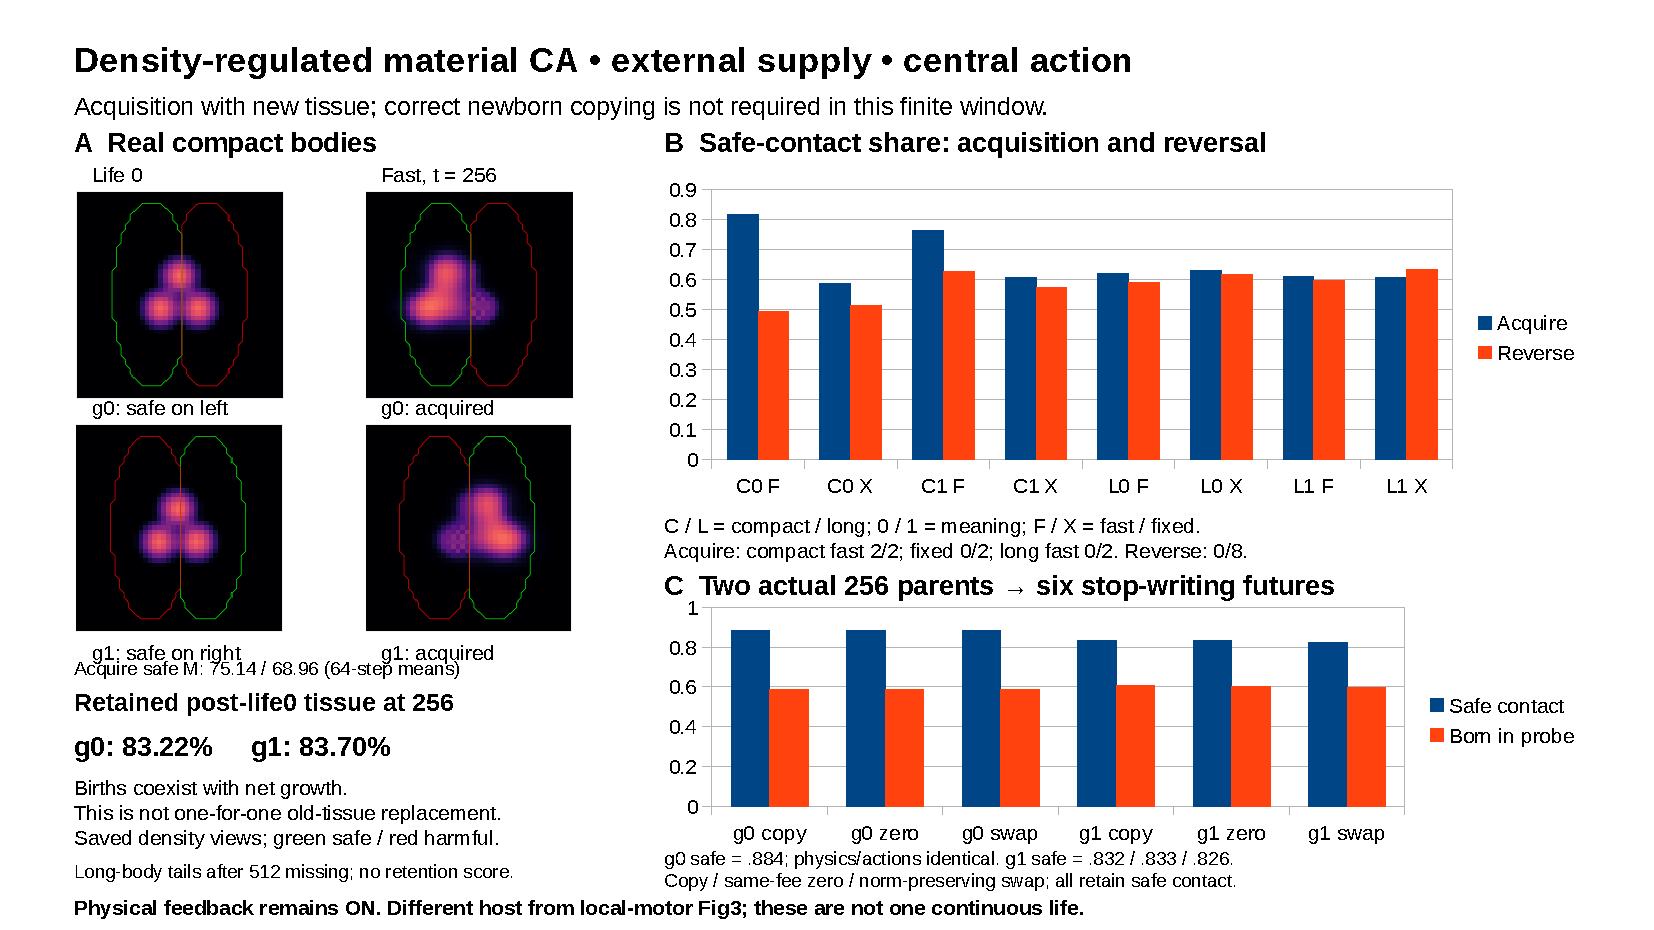
\includegraphics[width=\linewidth,height=0.72\textheight,keepaspectratio]{work/longform_v047/figures/young_turnover_v0475/young_turnover.pdf}
\captionsetup{font=footnotesize}
\caption{\textbf{Conditional acquisition during real tissue production in a distinct host.}
\textbf{a}, Actual compact density fields at life zero and acquired step 256. Green/red contours mark safe/harmful regions; these are density views, not spatial birth-cohort maps. Post-life-zero tissue constitutes $83.22\%$ and $83.70\%$ of the two acquired bodies. Births accompany net growth, so these shares do not measure one-for-one founder replacement.
\textbf{b}, Final-64 safe-contact fractions for all eight geometry--meaning--controller conditions. Compact fast acquisition passes $2/2$, compact fixed prior $0/2$, elongated fast $0/2$; all eight fail complete reversal. Success also requires absolute contact, viability and tissue criteria. The elongated expression tails after 512 are missing.
\textbf{c}, Two actual acquired parents each provide copy, same-tariff zero and norm-preserving swap futures. Writing stops for 128 steps, while physical energetic feedback continues. Safe contact is a final-64 mean; born-in-probe bars are endpoint retained fractions. All six related futures pass; the first parent's physical/action histories coincide. Correct newborn copying is therefore unnecessary in this tested window, with surviving old contents intact. This externally supplied density-regulated material CA has central action and differs from both original Lenia generation and the no-birth scalar-action host in Fig.~\ref{fig:scalar-action}.}
\label{fig:young-turnover}
\end{figure}





\subsection*{Sequential resource admission produces distinct mass and energy effects}

Regeneration depends on what a body can actually admit, not merely what its response function requests. In the resource experiments, a positive generative request passes through capacity and template constraints and then through precursor P and fuel F availability. We independently enable the registered transport capabilities in two acquired bodies, a porous form and a four-lobed form. Their first post-branch action is especially informative because the body, actual transport, licensed request and template support are still matched before the resource-admission paths separate.

At action 129, enabling P transport increases the requested mass subsequently rejected by F from $0.0786$ to $0.2863$ mass units in the porous body and from $0.1219$ to $0.2434$ mass units in the four-lobed body. The available F field is identical pointwise, and the independently evaluated F deficit remains unchanged, at $11.4326$ and $2.1079$, respectively. More requests reach the F constraint because the preceding P constraint has admitted more of them (Fig.~\ref{fig:allocation-feedback}). Increased downstream rejection therefore does not imply that the fuel supply itself became worse.

This is a general interpretive issue in a sequentially constrained system. A change in the mass rejected at one constraint can reflect the requests admitted by upstream constraints. The P and F deficits overlap and cannot be summed as independent lost masses. A scalar rejection amount would consequently be an ambiguous objective for an adaptive controller. The appropriate measurements include the admitted material, energy expenditure and the state on which each constraint acted, not just the rejected amount.

\begin{figure}[p]\centering
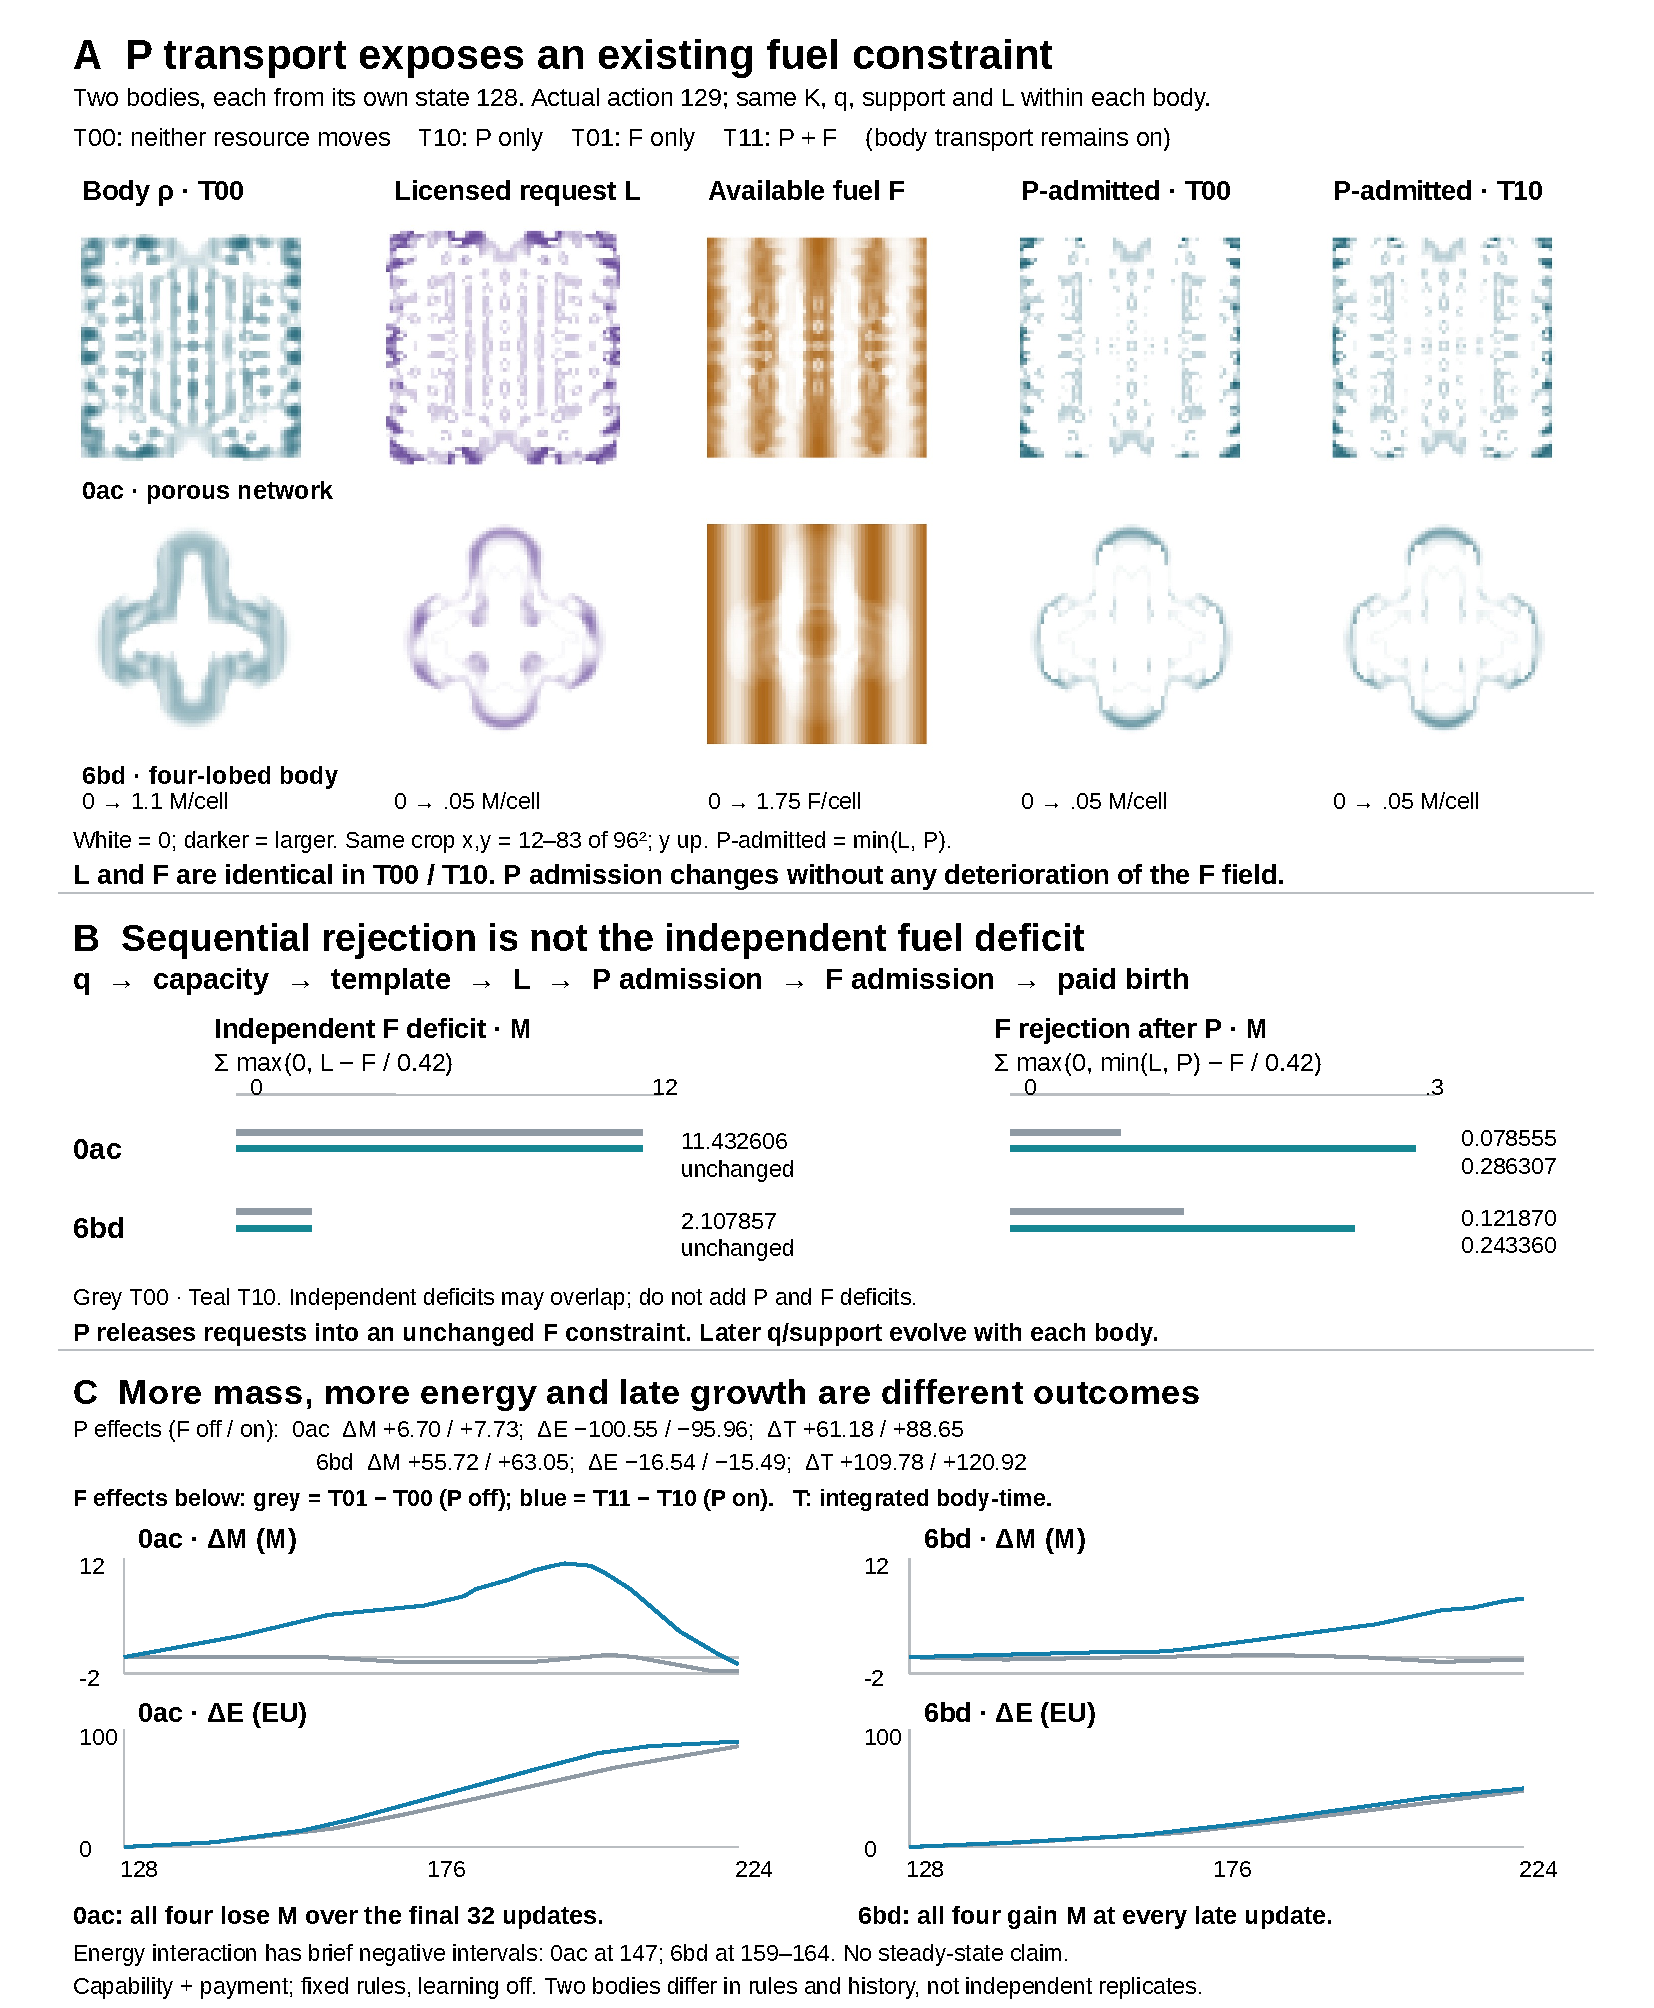
\includegraphics[width=\linewidth,height=.75\textheight,keepaspectratio]{figures/main/resource_constraints/resource_constraint_unmasking.pdf}
\caption{\textbf{P transport exposes fuel constraints without worsening fuel supply.}
\textbf{A,} Actual action 129 fields in two bodies continued from their own state 128. Fixed original-coordinate windows show T00 reference density, common licensed request $L$, common available fuel, and P-admitted requests with P transport off/on (T00/T10). Within each body, $K$, $q$, template support and $L$ match; F is identical pointwise.
\textbf{B,} The sequential capacity--template--P--F rule exposes more F rejection when P admits more requests, although the independent F deficit is unchanged. The quantities use separate scales; overlapping P/F deficits must not be added.
\textbf{C,} P increases final mass and body-time while reducing energy. Full-window F effects increase energy but change mass differently across bodies and time. All four 0ac branches lose mass over their final 32 updates; all four 6bd branches grow at every late update. Energy interaction is briefly negative despite positive endpoints. Capabilities and their actual payment change together; rules are fixed and learning is off. This is a conditional resource comparison, not an experience-adaptation test.}
\label{fig:allocation-feedback}\end{figure}


Over the subsequent window, P transport increases final mass and integrated body-time but lowers final energy. F transport raises energy throughout the tested interval, whereas its effect on mass depends on body and time. All four porous branches lose mass over their last 32 updates; all four four-lobed branches grow at each of those late updates. Even when endpoint interactions are positive, some energy interactions are briefly negative. Actual small starvation losses and the transport payments are retained in these accounts. No steady-state claim follows from the four-lobed late growth.

The matched first action permits a narrow mechanism statement about exposed constraints. It does not fix the organism over the entire future. Later density, templates, resource fields and transport masks differ, so a long-horizon effect cannot be interpreted as a single resource mediator acting in otherwise identical tissue. Capabilities and their actual costs change together. The experiment uses fixed rules with learning disabled; its role is to explain the physical opportunities and trade-offs that a future learner must control.

This distinction complements work on adaptive transport and collective resource organization\cite{tero,teronetwork,liu,prindle}. Such systems can show useful distributed organization without an explicit trial-based learning rule. Here, the accounting makes clear which resource constraint has changed and which consequences arise only after the body develops differently. It also supplies a reason to keep behaviour and viability separate: more tissue can be purchased with less residual energy, and less immediate growth can preserve fuel for a later useful action.


\subsection*{Acquired predictions alter actual maintenance, with a limited return under equal purchases}

The birth/death material CA allows a physical question that the conservative action tests cannot answer: can acquired experience change how a body protects tissue that is continually being produced and lost? We equip the externally supplied density-regulated host with a local protective reserve. Two initially neutral warning labels precede weak or strong mechanical contact. A standard conditional delta rule updates from the incident mechanical strain actually sensed during contact, including contact absorbed by protection. It does not receive a future damage field or the hidden label--strain relationship. The sensor thus measures an actual but relatively informative physical variable. Protection purchased from real precursor and old tissue energy is present before contact, absorbs demand and is depleted or lost with tissue (Fig.~\ref{fig:predictive-maintenance}).

Initial comparisons retain uniform, instantaneous and full fixed protection as well as the standard mean predictor and a higher-capacity risk predictor. The risk predictor's limited damage reduction accompanies additional protection and memory expense; no extra predictor advantage is established. Full fixed protection gives the lowest absolute loss with greater sustained investment. A later content test preserves the learned quantities and changes their readout: use the correct conditional content, pool the two labels, or exchange them. An initial attempted uniform-purchase match is limited by local capacity and payment, so it is not called equal purchasing. The actual equal-purchase test instead supplies a fixed common per-step quota that every branch realizes to floating-point precision.

From two complete acquired parents, correct conditional content reduces 96-step tissue injury from $5.43517$ to $4.53509$ and from $7.10679$ to $6.74210$ relative to pooled content, approximately 16.6\% and 5.1\%. Swapping content raises injury to $6.69137$ and $7.71390$. Correct content leaves more tissue and slightly more subsequent uptake in both parents. Its first terminal energy, however, is $90.61563$ versus $90.73901$ under pooling. Equal purchased protection and synthesis price do not equalize reserve holding, memory, movement or birth costs as bodies diverge. These finite comparisons show that already acquired conditional content can guide a useful physical allocation; they do not establish a new predictor, exclusive newborn plasticity or a general net benefit (the accompanying source-data tables).

\subsection*{Stronger physiology limits the benefit attributed to predictive maintenance}

We next restore the same two acquired parents and compare six policies under the same purchase allocator: continued delta learning, frozen learned content, each of two fixed label mappings, an immediate response to completed strain, and uniform allocation. Both fixed mappings are run unchanged in both worlds; we do not select the better mapping after seeing the hidden relation. The first 96 steps preserve that relation, then 96 steps introduce an unannounced change. Continued learning reduces post-change injury relative to frozen content by 9.17\% and 10.24\%. Nevertheless, it loses 7.51\% and 4.83\% more tissue than the immediate physiological response. Uptake, energy and mass provide no uniform post-change dominance over that response or uniform allocation. Improving over obsolete frozen content therefore does not establish that continued prediction is generally better than responsive physiology.

For readout comparison, all six policies carry and pay for the same four predictor/eligibility scalars, although fixed, instantaneous and uniform controls do not need all of them. This extra capacity charge makes those controls conservative economic comparators, not their cheapest possible implementations. Actual purchases are matched, but total expense remains state-dependent. The corresponding full 192-step injury advantage of delta over the immediate response is only about 1.27\% and 0.22\%, with opposing uptake and terminal-energy trade-offs. We retain all twelve paths and all three reporting windows (the accompanying source-data tables).

The registered tissue cohort supplies a second physical check. Tissue present at the complete parent is labelled before branching, and its actual removal by contact, starvation and rule death is tracked through material transport. Birth does not add to this old cohort. The strong-control futures retain about 70.5--75.4 units of later-born tissue while accumulating about 130.6--133.9 units of birth. These are different stocks and flows; neither high turnover nor continued protection identifies a causal requirement for correctly copied newborn content. The earlier newborn zero/swap outcomes remain relevant negative controls.

\subsection*{Contact timing changes the value of prepared reserves within a stable relationship}

A prospective timing intervention holds the learned warning relationship fixed. Two actual intermediate parents each supply four 96-step futures: frozen learned readout or immediate physiology, with a four-step distributed contact or its externally integrated strain concentrated into the first step. Warning, contact onset and interval remain matched. Predictive writing is disabled throughout, excluding different numbers of within-contact learning updates as the explanation. Bodies and later physical feedback can nevertheless diverge, so the intervention does not isolate event-time replenishment as a unique mediator.

Relative to immediate physiology, the learned readout reduces injury by 5.42\%/6.51\% for distributed contacts and 8.69\%/5.98\% for concentrated contacts. Uptake, final mass and final energy are slightly higher in all four conditions. Concentrating contact increases the absolute injury difference by $0.27094$ and $0.02758$ in the two parents; the second effect is small, and proportional benefit does not rise in both. These are finite benefits of ordinary delta-acquired content under a preserved relation, not successful learning of the previously changed relation (the accompanying source-data tables).

The physical distinction is informative. If every site had the same constant marginal avoidable loss $\beta$ and a common maintenance budget $B$ could always be usefully spent, total prevention would be $\beta B$, regardless of prediction accuracy. Here actual prevention is the sum of $\min(\text{reserve},\text{demand})$ over local contacts. Saturation, reserve decay, tissue loss and local capacity restrict when and where a purchase remains useful. The observations show a setting in which allocation and timing can matter, while the strong controls reveal how modest and conditional the realized benefit is. They do not partition all these physical causes or supply evidence for the uncompleted successor mechanism. The conservative learner and the regenerative maintenance body remain distinct experimental systems.

\begin{figure}[p]
\centering
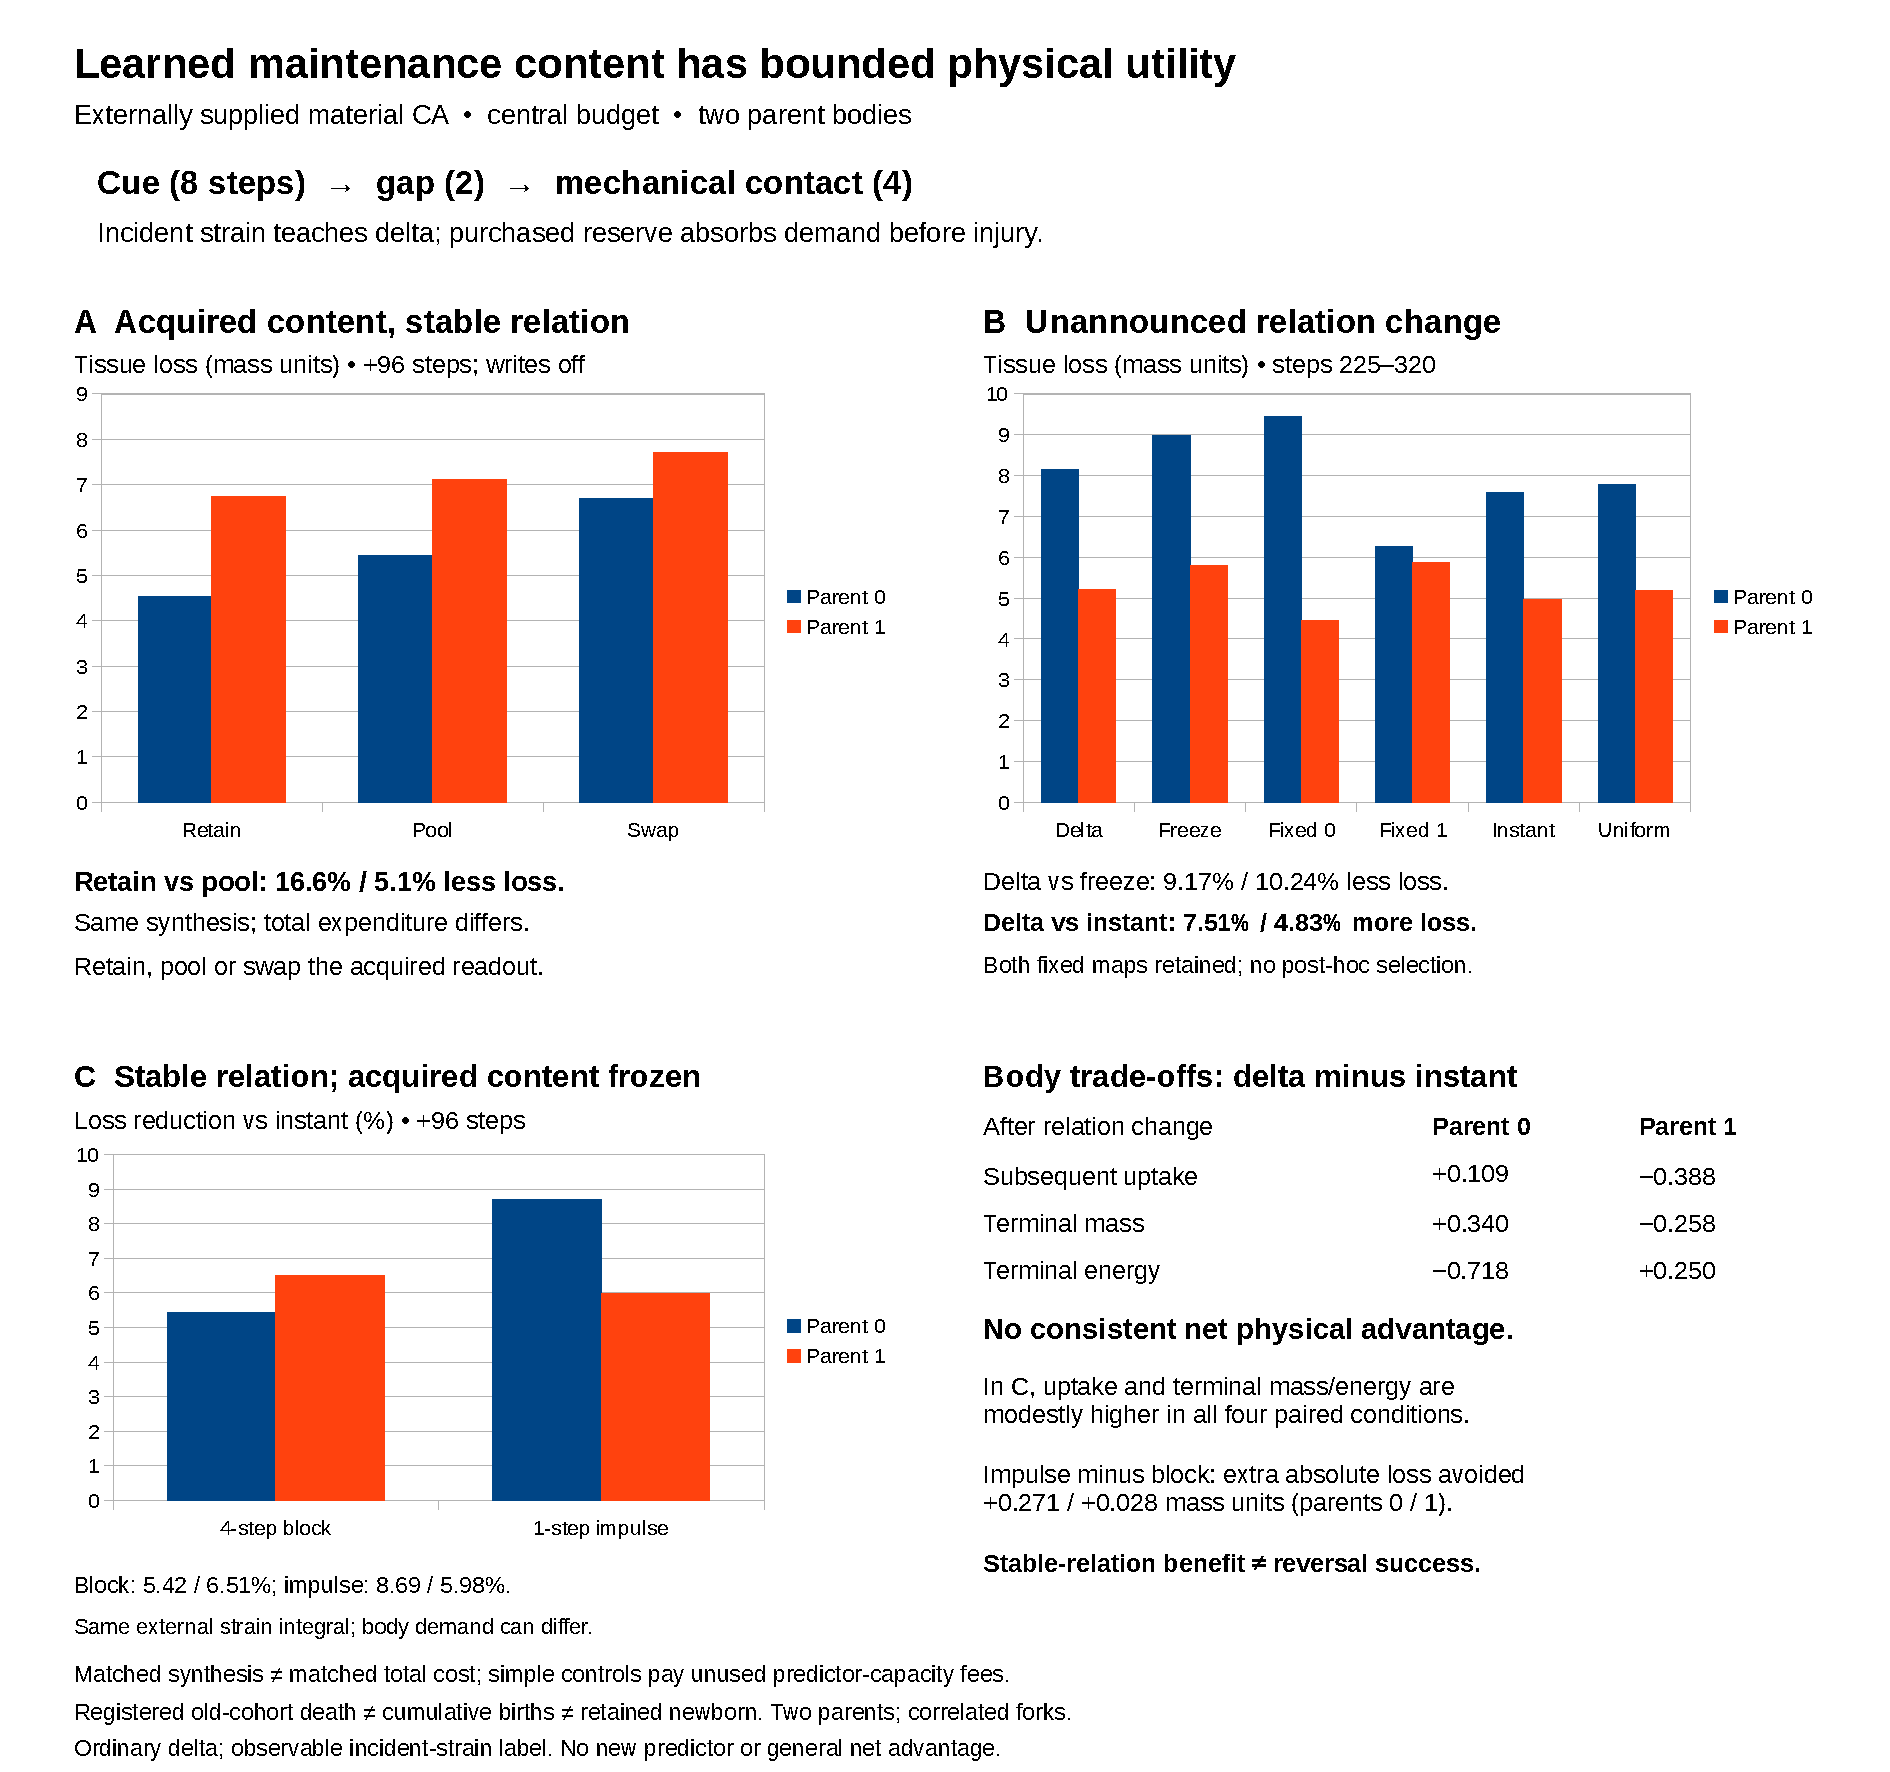
\includegraphics[width=\linewidth,height=0.63\textheight,keepaspectratio]{work/longform_v047/figures/predictive_maintenance_v048/predictive_maintenance.pdf}
\captionsetup{font=footnotesize}
\caption{\textbf{Acquired conditional maintenance has limited physical utility against strong instantaneous controls.}
The externally supplied, density-regulated material CA has centrally coordinated purchasing and a local incident-strain sensor. The ordinary conditional delta rule learns from completed contact, including strain absorbed by reserve; it is not a new predictor.
\textbf{a}, All three content readouts of two acquired parents over 96 new steps with writes stopped and the learned relation retained. Retaining rather than pooling content reduces injury by 16.6\%/5.1\% at equal realized reserve synthesis; swapping also raises injury.
\textbf{b}, All six policies from both actual parents. Bars show injury in steps 225--320 after the relation changes at boundary 224. Continued delta reduces injury relative to frozen content by 9.17\%/10.24\%, but loses 7.51\%/4.83\% more tissue than the instantaneous rule. Neither fixed map is selected retrospectively. The accompanying delta-minus-instantaneous contrasts show opposed uptake and terminal mass/energy effects, without consistent net benefit.
\textbf{c}, Two actual 192-step parents each supply four 96-step futures under the retained relation, crossing block/impulse contact with acquired/instantaneous readout; writes are frozen. External strain integrals match, while realized bodily demand can differ. Bars show paired injury reductions relative to instantaneous allocation. The impulse increases the absolute avoided-loss contrast by 0.271/0.028 mass units, but proportional benefit does not rise in both parents. This is a stable-relation expression test, not reversal success or isolation of one timing mediator.
Colours identify source parents within each assay; their branches are correlated conditions. Equal synthesis does not equalize total expenditure. Simple controls carry unused predictor capacity and its fees. Old-cohort death, cumulative birth and retained newborn tissue are distinct; none establishes newborn-content necessity. The original missing risk tail is not imputed. Full phase outcomes and physical accounts are in the accompanying maintenance source tables.}
\label{fig:predictive-maintenance}
\end{figure}


\section*{Discussion}
The experiments establish that experience can acquire content with a measurable physical function in cellular bodies. A local scalar-outcome rule forms a useful action direction without observing displacement or receiving a reward gradient. Controlled encounters support cue preference, reversal and a change in which earlier event predicts a consequence. In a birth/death host, conditional content can guide protection at equal realized purchases. These findings link internal updates to actual movement and tissue outcomes rather than treating an internal score as sufficient evidence of learning.

Their interpretation depends on three distinctions. The first is between acquiring content and supplying a capability. Motion axes, cohesion, sensors, exploration and transport are engineered in the scalar assay. Cue-gradient actuation is supplied in the association tests. The ordinary perturbation-response estimator, delta updates, eligibility traces and expert combination are established computational ideas\cite{sutton,florian,izhikevich,fremaux,williams,baxter}; their implementation in a deformable body does not establish a new learning algorithm. What the experiments add is a set of physical comparisons showing when these updates acquire something useful under stated interfaces.

The second distinction is between a content effect and a unique explanation of successful behaviour. Clearing or rotating an acquired direction changes later physical trajectories, yet one cleared body still passes its aftereffect. Its prior location and continued exploration remain consequential. Similarly, a fixed run-and-tumble response initialized with the acquired heading sustains useful action after execution changes, while a frozen estimate fails. Continued responsiveness is necessary in those futures, but continued fitting is not uniquely necessary. In the temporal assay, joint delta matches the gated experts, limiting any claim that the more elaborate architecture adds capacity.

The third distinction is between useful behaviour and sustained material benefit. The spatial-writing example shows an early mass advantage followed by greater starvation and a reversed final mass ordering. Sequential admission shows that more downstream rejection can result from relaxed upstream constraints without a worse fuel field. Energetic and collective accounts of motion help motivate these coupled measurements\cite{schweitzer,circle,tjhung,tonertu}; adaptive transport studies likewise show why useful organization should be assessed through its resource consequences\cite{tero,teronetwork,liu,prindle,alimflow,alimsignal,nakajima2015}. Neither increased mass nor greater retained energy is a universal substitute for the task actually being learned.

Conditional protection provides a positive but bounded example of this physical utility. Correctly using acquired warning content reduces injury relative to pooled or swapped content at equal protection purchases. Under a changed relationship, however, an immediate physiological response outperforms the continued predictor on injury. Under a stable relationship, prepared reserves yield small benefits whose magnitude depends on contact timing. Local saturation, reserve decay and changing tissue make equal purchase an informative control, but do not equalize every subsequent cost or isolate a single mediator.

The regenerative acquisition result also needs its negative intervention. Most material at the acquired compact checkpoints was born during the experiment, yet net growth means this fraction is not one-for-one replacement of founders. Correctly copying values into subsequent newborn tissue is unnecessary for passing the tested continuation while old contents remain. Tissue production and useful experience therefore coexist in this host, without demonstrating that memory has become independent of its original carriers. Reversal failures and unavailable terminal windows further restrict the result.

The main limitation is experimental scope. Two seeds or two acquired parents support a resolved case comparison, not broad generalization over environments, shapes or rules. Related mappings and dependent branches cannot increase that sample size. Some sensors, central readouts and external resource supplies remain installed and incompletely priced. No experiment presented here establishes lifelong adaptation, arbitrary environmental transfer or an advantage of a new optimizer. These limitations define the next substantive test: a single implementation must acquire and revise useful behaviour through repeated, measured material renewal, outperform equally informed physiological alternatives and retain its benefit under prespecified unfamiliar conditions. The present work supplies concrete mechanisms, counterexamples and reproducible comparisons for that test, rather than claiming its completion.

\section*{Methods}
\subsection*{Strictly scalar local action learning}

The primary action comparison uses the same conservative transport physics, with initial mass 24 and energy 144. Two noise seeds, 202610199431 and 202610199432, are paired with unknown physical rotations $+90^\circ$ and $-90^\circ$. The fixed periodic substrate is $0.6\sin(x)+0.4\sin(y)$ in the environment's spatial convention. Its coordinates and values are not policy inputs. A site with $\rho\geq10^{-4}$ can receive a completed payment; positive transfer is limited by local energy capacity and negative transfer by available energy. The policy observes
\begin{equation}
y_i=\frac{G_i-L_i}{0.005\rho_i}
\end{equation}
only where a nonzero transfer occurred. Normalization does not divide by field amplitude. Missing payments remain missing observations, not zero or adverse outcomes. The learning objective uses these environmental receipts; movement expenditure is reported separately and is not subtracted again to define the learner's scalar signal.

An internal eight-update oscillator controls exploration, without exposing the environmental schedule. At the start of each action block, the command is $\boldsymbol u=0.8\tanh(\boldsymbol m+0.6\boldsymbol\epsilon)$, with two independent standard Gaussian innovations. The command and score $\boldsymbol s=\boldsymbol\epsilon/0.6$, the starting scalar receipt and its validity flag travel with the material. An additional independent random heading field is generated on the same budget for all policies. The physical operator $K$ carries every extensive internal quantity using the same actual transported density. Its entries, donor displacement, velocity, spatial reward differences and the hidden actuator map are never passed to \texttt{choose} or \texttt{observe}. A transported indicator records whether actual motion was paid; this indicator supplies no motion direction.

At a completed block, a response update requires a current paid outcome, a valid transported starting observation and a completed-motion receipt. Using the transported score and starting observation, the fixed-rate response estimator is
\begin{equation}
\boldsymbol g\leftarrow(1-\beta)\boldsymbol g+
\beta\boldsymbol s\,(y_{\mathrm{end}}-y_{\mathrm{start}}),
\qquad \beta=1/8,\qquad \boldsymbol m=\operatorname{unit}(\boldsymbol g).
\end{equation}
The estimate starts at zero; zero norm gives zero mean. The rate was fixed before execution and not searched. The historical code label \texttt{spsa} denotes this single-trajectory perturbation-response rule. There are no paired simultaneous counterfactual evaluations, and forward material mixing prevents an interpretation as an unbiased whole-organism policy gradient. The rule estimates a reward-related action response, not an identified $2\times2$ mechanical mapping.

The accumulated policy updates a constant two-component mean with rate 2. Its context variant additionally reads its own current scalar and the previous completed block's scalar change; features are normalized and coefficients clipped to $[-2,2]$. Run-and-tumble retains its direction after an improving block and chooses a random heading after deterioration. The random policy writes no acquired direction. Response normalization, fixed-policy unit headings, command bound, noise and payment rules remain explicit: equal tariffs and exploration opportunities do not imply equal realized forces or costs. State storage and learning arithmetic have no additional physical tariff.

Life-zero trajectories comprise 320 acquisition steps, 320 steps with the reward meaning reversed and 128 steps with the same meaning but no new payments, reward observations or parameter writes. A phase passes only if its final-64-step mean field score exceeds 0.25, favourable mass fraction is at least 0.6, total mass is at least 12 and the largest connected fraction is at least 0.75. The full recorded stage and its failed criterion are retained even when a later phase passes. The two response-estimation lives are actual new runs under the frozen seeds and schedule; earlier four-policy data are reused read-only. 

Content probes restore the complete actual step-640 parents, preserve density, energy, other registrations, physical coupling, RNG and clock, then clear $\boldsymbol g$ or rotate it by $90^\circ$. All subsequent writes and outcome payments are disabled for 128 steps. Recorded retained tails supply the reference. The execution-change assay restores the complete step-320 parents; at step 321 the physical $\pm90^\circ$ map becomes the opposite $45^\circ$ map while reward meaning stays fixed. Each branch receives 320 paid steps and a 128-step aftereffect. The fixed run-and-tumble control is initialized with $\operatorname{unit}(\boldsymbol g)$ from that parent. Raw phase labels retain the recorder's word \texttt{reversal}, but this assay changes execution, not reward meaning. Frozen estimation stops only $\boldsymbol g$ updates: movement, lawful scalar feedback and transport continue. Source rows distinguish these interventions rather than pooling them under a common reversal success count.

\subsection*{Continuing-body cue assay}

The cue assay uses a periodic $32\times32$ lattice with density $\rho$, intracellular energy $E$, two cue values $Q_i$, a two-channel eligibility field $z_i$ and the most recently registered cue $\ell_i$. Initial total mass and energy are 24 and 72; cue values start at $0.2$. Two density-perturbation seeds, 202610197401 and 202610197402, are crossed with both initial cue--feedback orders. These four constructed conditions are evaluated with reactor, recent-feedback and eligibility policies under paired and unpaired exposures. There is no outer optimization in this batch.

The inherited material-transport model uses local four-neighbour movement, cohesion and pressure. Its fixed coefficients include time step $0.1$, cohesion 3, pressure 1.5, spatial scale 1.4 and cue gain 18. Local directed rates use a positive, bounded response to neighbour potential differences and to cue differences weighted by local values. The actual transported density and energy determine subsequent state; the external environment does not translate or reset the body between lessons. Movement and basal prices are $0.002$ and $0.012$ in the model's native units, with donor-energy limitations and capacity $4\rho$. The source implementation and complete coefficient file are retained rather than substituting a point-agent approximation for these dynamics.

At each actual transport, extensive amounts $\rho Q$, $\rho z$ and $\rho\ell$ travel with the recorded material operator $K$. Their intensive values are recovered using the corresponding transported mass, with zero-density entries masked. This registration is different from simply copying a value at its original lattice coordinate. Tissue may mix at a destination, so the resulting intensive average does not preserve distinct identities of all microscopic sources. No regenerative births occur in the cue assay.

Each step first executes the physical body update with its built-in plasticity disabled. The experiment then applies the prescribed local energy feedback to the resulting tissue. If $f$ is the signed external feedback field, the requested magnitude is $r=0.08\rho|f|$. Positive feedback deposits $g=\min(r,\max(4\rho-E,0))$; negative feedback removes $d=\min(r,E)$. Only the term appropriate to the sign is applied. The realized teaching signal is
\begin{equation}
y=\frac{g-d}{r},
\end{equation}
with zero where the denominator is absent. It therefore reports actual local delivered gain or loss, not the hidden environmental cue mapping. Normalization also means that very small nonzero feedback in a Gaussian tail can remain recognizable; this assay does not establish difficult credit assignment under a finite detection threshold.

All policies maintain the same sensory registrations. Where total current cue exceeds $0.05$, the normalized current cue replaces $\ell$. The eligibility field follows
\begin{equation}
z_i\leftarrow e^{-1/16}z_i+(1-e^{-1/16})c_i.
\end{equation}
Recent feedback uses $\phi=\ell$ and $\alpha=1$; eligibility uses $\phi=z/\sum_i z_i$ and $\alpha=0.5$. At sites with nonzero realized feedback and positive tissue, the update is
\begin{align}
\delta &=y-\sum_i Q_i\phi_i,\\
Q_i&\leftarrow\operatorname{clip}\left(Q_i+
\frac{\alpha\phi_i\delta}{\max(\sum_j\phi_j^2,10^{-12})},-1,1\right).
\end{align}
The reactor suppresses these writes while maintaining cue registrations and transport. There is no policy-gradient estimate\cite{williams,baxter}, no inferred outcome for an unobserved action and no learner input for phase, time, seed, coordinates or reversal identity. The supplied movement rule reads local values and local cue gradients. Extra learning arithmetic has no separately assigned physical price.


\subsection*{Exposure, reversal, probing and value erasure}

Each life lasts 960 updates. An initial 64-step probe is followed by two acquisition epochs. Each epoch contains a 48-step lesson for each cue and a 64-step unreinforced probe. A 64-step neutral interval and 64-step retention probe follow. The environmental mapping then reverses without informing the learner; two further lesson--probe epochs, another neutral interval and another retention probe complete the life. Probe endpoints are 64, 224, 384, 512, 672, 832 and 960.

During a lesson, a Gaussian cue of scale 6 is centred at the body's position at lesson onset and remains fixed there for that lesson. Cue presentation occupies the first 24 steps; four feedback pulses occur at offsets 32, 36, 40 and 44. Paired exposure uses a consistent sign for each cue within the current mapping. Unpaired exposure balances four positive and four negative pulses per cue across the two epochs, using the recorded seed shuffle in both mapping orders. Exposure is broad and imposed, rather than earned through free foraging. The environment uses the current centroid to place a new trial; the learner does not receive that centroid.

Probes place the two cue Gaussians at opposite offsets of four cells with scale 3.5, changing left--right placement across probes. No outcome feedback is delivered. Let $A_i$ be actual density integrated over the radius-2.5 contact region around cue $i$. The primary probe score is
\begin{equation}
p_{\rm correct}=\frac{A_{\rm currently\ positive}}{A_0+A_1}.
\end{equation}
The score is undefined when its denominator lacks support; no missing value is replaced by a successful response. We report endpoint fractions, condition-wise ranges and descriptive condition means. They are distinct from time-averaged probe contact or signed centroid displacement, which remain in the source tables.

The reversal occurs at the 512 boundary. The first new completed feedback is at 545, and the first post-reversal behavioural probe spans 609--672. By that probe the body has received four feedback pulses for each cue. Recovery is therefore established by the first measured post-exposure probe, not after one feedback event. Choice during forced exposure is not reconstructed as an independent error rate.

Each 960-step terminal state supplies two 64-step unreinforced continuations. Both disable value writes. The retained branch keeps $Q$, and the erased branch sets $Q_i=0.2$ while preserving density, energy, eligibility and last-cue records exactly at branching. Transport and sensing continue. These paired forks measure expression under the remaining bodily state; they do not erase the entire acquisition history. Viability requires mass at least 12 and a largest connected component containing at least half the mass, without 32 consecutive failing updates. The final report contains 24 main lives and 48 forks, all alive; pilot trajectories are separate. Its total accounting includes 28,032 actual updates across science and pilots, whereas the 72 scientific paths comprise 26,112 updates. No trajectory was rerun for this manuscript's summary.


\subsection*{Distractor histories and changing temporal sources}

The temporal-credit experiment uses two additional seeds, 202610197403 and 202610197404, with both initial cue-meaning orders. Twenty lives begin under five rules. Each 40-step lesson presents an earlier cue for eight steps, a four-step gap, a recent cue for eight steps and another four-step gap; feedback is delivered at completed updates 25, 29, 33 and 37. Each four-lesson block traverses the full earlier--recent cue cross in randomized order. Local cue onsets update two event registers, which travel with the material through the same actual transport as the body. All arms maintain the same auxiliary fields; their rules differ in how those available records are used. Neither the temporal source nor a hidden cue label is passed to a learner.

Let $r_0,r_1$ be the two-component recent and earlier cue registers, and $b_0,b_1$ their associated coefficient vectors. Recent-cue, fixed-trace and fixed-earlier delta use the normalized update above with learning rate one and the respective feature. The fixed trace retains the exponential time constant of sixteen updates. Joint delta uses the concatenated four-component feature and prediction $\hat y=\sum_{j=0}^1 b_j\cdot r_j$ in a normalized least-mean-squares update. For gated experts, the two pre-update predictions are $\hat y_j=b_j\cdot r_j$, and each expert receives its own normalized unit-rate delta update. At sites with nonzero realized feedback, the earlier-source log weight changes according to
\begin{equation}
g\leftarrow\operatorname{clip}\bigl(0.99g+0.75[(\hat y_0-y)^2-(\hat y_1-y)^2],-8,8\bigr),
\qquad w=(1+e^{-g})^{-1}.
\end{equation}
The motor readout uses $(1-w)b_0+wb_1$ for the gated rule and $b_0+b_1$ for joint delta, clipped to $[-1,1]$. The weight is updated from prediction errors computed before the coefficient updates; it is not supplied with the true lag. These calculations add no native bodily step and carry no separately priced arithmetic or storage cost.

The initial distractor experiment lasts 1216 steps for surviving bodies and includes six fixed acquisition, cue-meaning reversal and retention probes. A complete behavioural pass requires each endpoint contact fraction to be at least $0.65$ and the body to survive. The three connectivity failures stop their lives; unobserved probes and terminal forks are not generated. At clock 1216, the seventeen surviving full states are loaded exactly for a 576-step continuation. Cue meanings remain fixed while the recent event replaces the earlier event as feedback source. Each rule continues its own actual prior body and state. The first changed-source feedback is at continuous clock 1241 and the first new probe spans 1377--1440, after sixteen pulses. Two four-lesson blocks with probes are followed by a neutral interval and retention probe. Endpoint contact fractions use the radius-2.5 regions defined above, not Gaussian-cue intensity weights or time-averaged accuracy.


\subsection*{Spatial writing and matched-state interventions}

The earlier spatial-writing example branches at step 240 from identical acquired body and remaining world. Stopping new writing leaves decay, transport, eligibility and subsequent local movement active. Saved fields use original periodic coordinates and common scales. Density masks specify tissue support, not confidence in an inferred value. The local-state and specific-energy panels are observations of evolving fields; they are not separate interventions on those fields. The full 61-point path is retained along with distinct injury and starvation accounts. This model also has no birth. Full source-specific formulas appear in the accompanying detailed protocols.


\subsection*{Resource-constrained generation}

In the generative models, a signed rule response separates deletion from requested production. Positive production is limited by spatial capacity, a local template and actual precursor P and fuel F. The admission order is retained, so a conditional downstream rejection is not equated with an independent deficit evaluated before upstream restriction. Negative response removes actual tissue and its associated energy. Resource transport, uptake, pumping, deletion and conversion have the costs and sinks recorded by that model. External interventions that coordinate requests or exchange resource packages are labelled explicitly; their extra computation or external work is not silently charged to the organism.


\subsection*{Density-regulated regeneration with energetic consequences}

This host uses actual material transport and the existing paid local conversion constraints, while replacing the kernel-derived generative request with a fixed density rule. With physical step $dt=0.05$, rule death removes $0.005$ times the post-actor body, and the requested birth is $0.015$ times the local $3\times3$ binomial-weighted survivor average, with weights $[1,2,1]\otimes[1,2,1]/16$, times $[1-\rho_{\mathrm{survivor}}/0.8]_+$. Actual admission still obeys local $P/F$ support and energy prices. Old dual-kernel metadata supplies grid size and clock but not the generative rate. A uniform external bath restores local $P$ and $F$ to $0.2$ before each native step; actual additions are logged. The apparatus and central computation are unpriced, so this is not a closed metabolism.

Two initial geometry recipes, compact and elongated, each have both initial outcome meanings, with shared within-condition physical states and exploration tapes for fast and fixed-prior controls. Founder energy is $1.8M$ in both controls. Two Gaussian cues at $(x,y)=(26,32)$ and $(38,32)$ use widths $5$ and $12$ with an explicit winner-take-local partition, avoiding simultaneous cue aliasing. A central five-action readout and fixed motor gain $0.45$ are installed. Bounded current-cue learning uses $\alpha=1$; the prior control never writes acquired values but retains sensing, transport, maintenance and copying. Actual uptake is followed, before generation, by a local energy tax of $0.4$ per physical time per old mass in the relevant region. Only the affordable amount enters heat; feedback uses actual uptake minus this paid tax. Unpaid tax is not fictitious negative feedback, and cue identity does not directly delete tissue.

The main schedule is acquisition through 256, unannounced outcome reversal through 512, then stop-writing expression through 640 with physical outcomes continuing. Four actual fast-256 parents also supply paired frozen-writing reversal continuations to 512; the matching fast futures are reused read-only. Survival requires $M\ge0.5M_0$, a largest connected component (density threshold $0.02$) of at least $0.8$ of body mass, and at most $0.01$ in the two-cell border. The final 64 updates of a behavioural phase require mean safe-contact mass at least 8, safe fraction at least $0.65$, and actual new-tissue fraction at least $0.1$. The contact measure is specific to the exclusive cue regions and differs from both the local-motor field score and the earlier radius-2.5 contact assay. Missing terminal windows have no evaluated fraction or pass outcome in the manuscript tables.

Only the two acquired compact states qualify for the newborn-content probe. From the same complete actual-256 parent, writers stop and meaning stays unchanged for 128 updates. At actual birth, copied pre-write local contents are retained, zeroed under the same tariff, or swapped between cue channels with their norm preserved. Zeroing is not norm matched. Old tissue values remain unchanged at the intervention; newborn personal registrations, seen flags, traces and pending state begin at zero. Holding requests $0.00005$ energy units per unit of old mass per step. Copying requests $0.002$ energy units per unit of actually admitted newborn mass; realized payments are energy-limited. Denied charges remain explicit, and realized later fees can differ as futures diverge. Sensing, physical outcomes and transport continue. Material labels record tissue actually born since life zero and since the probe branch; they are not estimates of one-to-one founder replacement when body mass also grows.






\subsection*{Predictive maintenance and equal-purchase physical controls}

The maintenance series uses the explicitly supplied density-regulated birth/death host described above. Local precursor and fuel are restored to 0.2 before each update, with actual additions logged. Protection transfers real precursor into a reserve, costs 0.3 units of old intracellular energy per unit synthesized, incurs holding cost 0.001 per reserve unit per step and decays by 3\% per step. Total local capacity is 0.08 times current tissue, local production is limited to 0.008 times tissue per step, and the initial common production rate is 0.004 times total mass. Realized production is further limited by precursor and payable old energy. Loss of reserve and tissue is registered in waste and dead-energy accounts.

Two neutral warning channels are shown for eight steps, followed by two silent steps and four steps of actual mechanical contact. In the initial jittered protocol, contact onsets are separated by 22--27 steps. Spatial halves receive weak strain 0.002 or strong strain drawn from 0.012/0.024; cue identity predicts which side receives stronger contact. The learner reads current warning and completed incident mechanical strain, including strain absorbed by protection. This is supplied mechanical sensing, not inference of a counterfactual unprotected injury. Tissue demand is $\rho\,\mathrm{strain}$, absorbed amount is the lesser of reserve and demand, and residual demand removes actual tissue and its energy. Damage precedes learning and new purchasing. No future strain map, relation-change flag or absolute environment clock enters the learner.

Local cue registrations and conditional estimates move with actual material transport. Standard delta learning updates two conditional means only at actual contact. Its four charged scalars include the registrations; the risk variant additionally stores second moments and pays for six. Newborn registrations start at zero, while pre-write conditional content is copied from surviving donors subject to the actual charge. Earlier incomplete runs and unmatched-purchase controls are retained in the source records; only the completed, actually matched assays support the equal-purchase comparisons.

The subsequent equal-purchase assay fixes each per-step quota at 0.0015 times registered parent mass and distributes it using $\rho(0.002+\text{conditional estimate})$ subject to the same capacity and payment constraints. Correct, pooled and swapped readouts retain the same stored quantities and tariffs. All six branches actually realize the shared quota; their three 96-step futures per acquired parent total 576 updates. Equal synthesis is not equal total expense, because holding, movement, copying and births respond to each physical future.

The strong-physiology assay restores two actual delta step-128 parents and applies six policies for 192 steps each. The warning relationship changes after the first 96 steps. This follow-up uses fixed 24-step onset spacing, with four contacts before and four after the change (warning starts 132, 156, 180, 204, 228, 252, 276 and 300). Continued delta, frozen content, each fixed mapping, immediate response to completed strain and uniform allocation share the same quota allocator and four charged scalars. Both fixed mappings are evaluated unchanged in both worlds. Their redundant predictor capacity is an explicit charge to simple controls, precluding claims of economic dominance over a minimal implementation. A passive cohort labels all tissue present at branching and is transported and removed by the actual physical operators; newborns never enter this registered old cohort. Stage deaths are normalized by registered parent mass, not by surviving tissue alone.

The timing assay uses two actual step-192 parents from that strong-control series. Frozen learned and instantaneous readouts each receive a 96-step future under distributed four-step contact or a single concentrated contact with the same per-cell integrated external strain. Warning starts are 196, 220, 244 and 268: four contacts per 96-step future at fixed 24-step spacing. Onset and warning are matched, and prediction remains frozen. The impulse applies four times the strain only at warning-start plus ten, replacing the four-step contact block. The environment changes the time profile; the learner senses only current stimuli. Equal external strain does not imply equal realized bodily demand when tissue and later motion diverge. All twenty futures complete; the maximum per-step purchase mismatch is $5.55\times10^{-17}$. The supply apparatus, sensor implementation, central budget coordination and computation remain incompletely priced. None of these branches is an independent replication of a new learned life.

\subsection*{Analysis and reproducibility}
Comparisons are descriptive and use the specified trajectory or complete-parent units. Opposite mappings, repeated phases, material sites and branches of one parent are not independent replicates. No population-level significance or general superiority is inferred from the two-parent mechanism tests. Missing outcomes are not imputed, later successes do not replace earlier failures, and realized costs are reported separately from behavioural criteria. A changed state can influence action without being the sole explanation of successful occupancy.

The seven main figures reuse their existing, editable presentation sources and verified simulation exports. No new simulation or illustration was generated for this editorial revision. Display scales, coordinate conventions, masks and paired comparisons are stated in the figure legends. Exact configurations, seeds and necessary initial conditions accompany the final code; figure data and original detailed protocols remain within this Article. These files retain the full precision and accounting needed beyond the rounded quantities in the main text.

\section*{Data and code availability}
The final implementation, comparison rules, configurations, required initial states and random seeds are registered as Repo \texttt{repo\_bd47ffeac5c8}. Figure exports and their corresponding editable PPTX files remain in this Article's figure directories. The source-data index \path{data/index.json} maps historical experiment paths to the retained files in \path{data/objects/}. Detailed condition tables and protocols accompany the Article as source files; they are separate supporting material and are not appended to the main PDF. The seven main figures reuse verified results without new simulation. Selected animation and learning demonstrations remain available in the project workbench.
\section*{Author contributions and competing interests}
Authorship, contributor roles and competing-interest declarations require confirmation by the research contributors before submission.
\let\sharedbibliographyend\endthebibliography
\renewcommand{\endthebibliography}{%
\bibitem{nakajima2015} Nakajima, K., Hauser, H., Li, T. \& Pfeifer, R. Information processing via physical soft body. \textit{Scientific Reports} \textbf{5}, 10487 (2015). \href{https://doi.org/10.1038/srep10487}{doi:10.1038/srep10487}.
\bibitem{pdnca} Zhang, I., Risi, S. \& Darlow, L. Petri Dish NCA. Late Breaking Abstract (2025). \url{https://pub.sakana.ai/pdnca/assets/pdf/pdnca.pdf}. Author project page: \url{https://pub.sakana.ai/pdnca/}.
%
\sharedbibliographyend}
\begin{thebibliography}{99}
\bibitem{chan} Bert Wang-Chak Chan. Lenia: Biology of Artificial Life. \emph{Complex Systems} 28, 251--286 (2019). \url{https://doi.org/10.25088/ComplexSystems.28.3.251}.
\bibitem{expandedlenia} Chan, B. W.-C. Lenia and Expanded Universe. In \emph{The 2020 Conference on Artificial Life}, 221--229 (2020). \url{https://doi.org/10.1162/isal_a_00297}.
\bibitem{hamon} Hamon, G., Etcheverry, M., Chan, B. W.-C., Moulin-Frier, C. \& Oudeyer, P.-Y. Discovering sensorimotor agency in cellular automata using diversity search. \emph{Sci. Adv.} \textbf{11}, eadp0834 (2025). \href{https://doi.org/10.1126/sciadv.adp0834}{doi:10.1126/sciadv.adp0834}.
\bibitem{plantec} Plantec, E. et al. Flow-Lenia: Emergent evolutionary dynamics in mass conservative continuous cellular automata. \emph{Artif. Life} \textbf{31}, 228--248 (2025). \href{https://doi.org/10.1162/artl_a_00471}{doi:10.1162/artl\_a\_00471}.
\bibitem{asal} Kumar, A. et al. Automating the Search for Artificial Life With Foundation Models. \emph{Artificial Life} \textbf{31}, 368--396 (2025). \url{https://doi.org/10.1162/artl.a.8}.
\bibitem{growingca} Alexander Mordvintsev, Ettore Randazzo, Eyvind Niklasson and Michael Levin. Growing Neural Cellular Automata. \emph{Distill} 5 (2020). \url{https://doi.org/10.23915/distill.00023}.
\bibitem{developmental} D\'{a}niel L. Barab\'{a}si, Taliesin Beynon, \'{A}d\'{a}m Katona and Nicolas Perez-Nieves. Complex computation from developmental priors. \emph{Nature Communications} 14, 2226 (2023). \url{https://doi.org/10.1038/s41467-023-37980-1}.
\bibitem{bricks} Rodrigo Moreno, Andr\'{e}s Fa\'{i}\~{n}a, Shyam Sudhakaran, Kathryn Walker and Sebastian Risi. Smart cellular bricks for decentralized shape classification and damage recovery. \emph{Nature Communications} 17, 5932 (2026). \url{https://doi.org/10.1038/s41467-026-75166-7}.
\bibitem{gupta2021} Gupta, A., Savarese, S., Ganguli, S. \& Fei-Fei, L. Embodied intelligence via learning and evolution. \emph{Nat. Commun.} \textbf{12}, 5721 (2021). \url{https://doi.org/10.1038/s41467-021-25874-z}.
\bibitem{duan} Duan, Y. et al. RL$^2$: Fast reinforcement learning via slow reinforcement learning. Preprint at \url{https://arxiv.org/abs/1611.02779} (2016).
\bibitem{wang} Wang, J. X. et al. Learning to reinforcement learn. Preprint at \url{https://arxiv.org/abs/1611.05763} (2016).
\bibitem{miconi} Miconi, T., Clune, J. \& Stanley, K. O. Differentiable plasticity: training plastic neural networks with backpropagation. \emph{Proc. Mach. Learn. Res.} \textbf{80}, 3559--3568 (2018).
\bibitem{backpropamine} Thomas Miconi, Aditya Rawal, Jeff Clune and Kenneth O. Stanley. Backpropamine: training self-modifying neural networks with differentiable neuromodulated plasticity. \emph{International Conference on Learning Representations} (2019). \url{https://openreview.net/forum?id=r1lrAiA5Ym}.
\bibitem{khajehabdollahi} Khajehabdollahi, S., Giannakakis, E., Buendia, V., Martius, G. \& Levina, A. Locally adaptive cellular automata for goal-oriented self-organization. Preprint at \url{https://arxiv.org/abs/2306.07067} (2023).
\bibitem{boisseau} Romain P. Boisseau, David Vogel and Audrey Dussutour. Habituation in non-neural organisms: evidence from slime moulds. \emph{Proceedings of the Royal Society B: Biological Sciences} 283, 20160446 (2016). \url{https://doi.org/10.1098/rspb.2016.0446}.
\bibitem{reid} Chris R. Reid, Tanya Latty, Audrey Dussutour and Madeleine Beekman. Slime mold uses an externalized spatial ``memory'' to navigate in complex environments. \emph{Proceedings of the National Academy of Sciences} 109, 17490--17494 (2012). \url{https://doi.org/10.1073/pnas.1215037109}.
\bibitem{kramar2021} Kramar, M. \& Alim, K. Encoding memory in tube diameter hierarchy of living flow network. \emph{Proc. Natl Acad. Sci. USA} \textbf{118}, e2007815118 (2021). \url{https://doi.org/10.1073/pnas.2007815118}.
\bibitem{reiber} H. Reiber and A. F. Nogueira J\'{u}nior. Missing evidence for memory in the monocellular slime mold. \emph{Proceedings of the National Academy of Sciences} 118, e2105928118 (2021). \url{https://doi.org/10.1073/pnas.2105928118}.
\bibitem{dunlap2009} Dunlap, A. S. \& Stephens, D. W. Components of change in the evolution of learning and unlearned preference. \emph{Proc. R. Soc. B} \textbf{276}, 3201--3208 (2009). \url{https://doi.org/10.1098/rspb.2009.0602}.
\bibitem{vogel} David Vogel and Audrey Dussutour. Direct transfer of learned behaviour via cell fusion in non-neural organisms. \emph{Proceedings of the Royal Society B: Biological Sciences} 283, 20162382 (2016). \url{https://doi.org/10.1098/rspb.2016.2382}.
\bibitem{boussard} A. Boussard, J. Delescluse, A. P\'{e}rez-Escudero and A. Dussutour. Memory inception and preservation in slime moulds: the quest for a common mechanism. \emph{Philosophical Transactions of the Royal Society B: Biological Sciences} 374, 20180368 (2019). \url{https://doi.org/10.1098/rstb.2018.0368}.
\bibitem{acar} Murat Acar, Attila Becskei and Alexander van Oudenaarden. Enhancement of cellular memory by reducing stochastic transitions. \emph{Nature} 435, 228--232 (2005). \url{https://doi.org/10.1038/nature03524}.
\bibitem{micheelsen} Mille A Micheelsen, Namiko Mitarai, Kim Sneppen and Ian B Dodd. Theory for the stability and regulation of epigenetic landscapes. \emph{Physical Biology} 7, 026010 (2010). \url{https://doi.org/10.1088/1478-3975/7/2/026010}.
\bibitem{shomrat} Tal Shomrat and Michael Levin. An automated training paradigm reveals long-term memory in planaria and its persistence through head regeneration. \emph{Journal of Experimental Biology} 216, 3799--3810 (2013). \url{https://doi.org/10.1242/jeb.087809}.
\bibitem{yang} Chih-Yu Yang, Maja Bialecka-Fornal, Colleen Weatherwax, Joseph W. Larkin, Arthur Prindle, Jintao Liu, Jordi Garcia-Ojalvo and G\"{u}rol M. S\"{u}el. Encoding Membrane-Potential-Based Memory within a Microbial Community. \emph{Cell Systems} 10, 417--423.e3 (2020). \url{https://doi.org/10.1016/j.cels.2020.04.002}.
\bibitem{lambert} Guillaume Lambert and Edo Kussell. Memory and Fitness Optimization of Bacteria under Fluctuating Environments. \emph{PLoS Genetics} 10, e1004556 (2014). \url{https://doi.org/10.1371/journal.pgen.1004556}.
\bibitem{mitchell} Amir Mitchell, Gal H. Romano, Bella Groisman, Avihu Yona, Erez Dekel, Martin Kupiec, Orna Dahan and Yitzhak Pilpel. Adaptive prediction of environmental changes by microorganisms. \emph{Nature} 460, 220--224 (2009). \url{https://doi.org/10.1038/nature08112}.
\bibitem{tagkopoulos} Ilias Tagkopoulos, Yir-Chung Liu and Saeed Tavazoie. Predictive Behavior Within Microbial Genetic Networks. \emph{Science} 320, 1313--1317 (2008). \url{https://doi.org/10.1126/science.1154456}.
\bibitem{mery2005} Mery, F. \& Kawecki, T. J. A cost of long-term memory in Drosophila. \emph{Science} \textbf{308}, 1148 (2005). \url{https://doi.org/10.1126/science.1111331}.
\bibitem{alimflow} Karen Alim, Gabriel Amselem, Fran\c{c}ois Peaudecerf, Michael P. Brenner and Anne Pringle. Random network peristalsis in Physarum polycephalum organizes fluid flows across an individual. \emph{Proceedings of the National Academy of Sciences} 110, 13306--13311 (2013). \url{https://doi.org/10.1073/pnas.1305049110}.
\bibitem{alimsignal} Karen Alim, Natalie Andrew, Anne Pringle and Michael P. Brenner. Mechanism of signal propagation in Physarum polycephalum. \emph{Proceedings of the National Academy of Sciences} 114, 5136--5141 (2017). \url{https://doi.org/10.1073/pnas.1618114114}.
\bibitem{liu} Jintao Liu, Arthur Prindle, Jacqueline Humphries, Mar\c{c}al Gabalda-Sagarra, Munehiro Asally, Dong-yeon D. Lee, San Ly, Jordi Garcia-Ojalvo and G\"{u}rol M. S\"{u}el. Metabolic co-dependence gives rise to collective oscillations within biofilms. \emph{Nature} 523, 550--554 (2015). \url{https://doi.org/10.1038/nature14660}.
\bibitem{prindle} Arthur Prindle, Jintao Liu, Munehiro Asally, San Ly, Jordi Garcia-Ojalvo and G\"{u}rol M. S\"{u}el. Ion channels enable electrical communication in bacterial communities. \emph{Nature} 527, 59--63 (2015). \url{https://doi.org/10.1038/nature15709}.
\bibitem{schweitzer} Frank Schweitzer, Werner Ebeling and Benno Tilch. Complex Motion of Brownian Particles with Energy Depots. \emph{Physical Review Letters} 80, 5044--5047 (1998). \url{https://doi.org/10.1103/PhysRevLett.80.5044}.
\bibitem{circle} van Teeffelen, S. \& L\"owen, H. Dynamics of a Brownian circle swimmer. \emph{Phys. Rev. E} \textbf{78}, 020101(R) (2008). \url{https://doi.org/10.1103/PhysRevE.78.020101}.
\bibitem{tonertu} Toner, J. \& Tu, Y. Flocks, herds, and schools: A quantitative theory of flocking. \emph{Phys. Rev. E} \textbf{58}, 4828--4858 (1998). \url{https://doi.org/10.1103/PhysRevE.58.4828}.
\bibitem{tjhung} Elsen Tjhung, Davide Marenduzzo and Michael E. Cates. Spontaneous symmetry breaking in active droplets provides a generic route to motility. \emph{Proceedings of the National Academy of Sciences} 109, 12381--12386 (2012). \url{https://doi.org/10.1073/pnas.1200843109}.
\bibitem{tero} Atsushi Tero, Ryo Kobayashi and Toshiyuki Nakagaki. A mathematical model for adaptive transport network in path finding by true slime mold. \emph{Journal of Theoretical Biology} 244, 553--564 (2007). \url{https://doi.org/10.1016/j.jtbi.2006.07.015}.
\bibitem{teronetwork} Atsushi Tero, Seiji Takagi, Tetsu Saigusa, Kentaro Ito, Dan P. Bebber, Mark D. Fricker, Kenji Yumiki, Ryo Kobayashi and Toshiyuki Nakagaki. Rules for Biologically Inspired Adaptive Network Design. \emph{Science} 327, 439--442 (2010). \url{https://doi.org/10.1126/science.1177894}.
\bibitem{duran} Salva Duran-Nebreda, Adriano Bonforti, Ra\'{u}l Monta\~{n}ez, Sergi Valverde and Ricard Sol\'{e}. Emergence of proto-organisms from bistable stochastic differentiation and adhesion. \emph{Journal of The Royal Society Interface} 13, 20160108 (2016). \url{https://doi.org/10.1098/rsif.2016.0108}.
\bibitem{colizzi} Enrico Sandro Colizzi, Renske MA Vroomans and Roeland MH Merks. Evolution of multicellularity by collective integration of spatial information. \emph{eLife} 9, e56349 (2020). \url{https://doi.org/10.7554/eLife.56349}.
\bibitem{kriegman} Sam Kriegman, Nick Cheney, Francesco Corucci and Josh C. Bongard. Interoceptive robustness through environment-mediated morphological development. \emph{Proceedings of the Genetic and Evolutionary Computation Conference}, 109--116 (2018). \url{https://doi.org/10.1145/3205455.3205529}.
\bibitem{predictability} Lars Koopmans, Elinor M. Kay and Hyun Youk. Predictability can be dynamically constructed in deterministic systems. \emph{Nature Communications} 17, 10720 (2026). \url{https://doi.org/10.1038/s41467-026-77737-0}.
\bibitem{florian} R\u{a}zvan V. Florian. Reinforcement Learning Through Modulation of Spike-Timing-Dependent Synaptic Plasticity. \emph{Neural Computation} 19, 1468--1502 (2007). \url{https://doi.org/10.1162/neco.2007.19.6.1468}.
\bibitem{izhikevich} E. M. Izhikevich. Solving the Distal Reward Problem through Linkage of STDP and Dopamine Signaling. \emph{Cerebral Cortex} 17, 2443--2452 (2007). \url{https://doi.org/10.1093/cercor/bhl152}.
\bibitem{fremaux} Nicolas Fr\'{e}maux, Henning Sprekeler and Wulfram Gerstner. Functional Requirements for Reward-Modulated Spike-Timing-Dependent Plasticity. \emph{The Journal of Neuroscience} 30, 13326--13337 (2010). \url{https://doi.org/10.1523/JNEUROSCI.6249-09.2010}.
\bibitem{sutton} Richard S. Sutton. Learning to predict by the methods of temporal differences. \emph{Machine Learning} 3, 9--44 (1988). \url{https://doi.org/10.1007/BF00115009}.
\bibitem{williams} Ronald J. Williams. Simple statistical gradient-following algorithms for connectionist reinforcement learning. \emph{Machine Learning} 8, 229--256 (1992). \url{https://doi.org/10.1007/BF00992696}.
\bibitem{baxter} J. Baxter and P. L. Bartlett. Infinite-Horizon Policy-Gradient Estimation. \emph{Journal of Artificial Intelligence Research} 15, 319--350 (2001). \url{https://doi.org/10.1613/jair.806}.
\bibitem{agarwal2021} Agarwal, R., Schwarzer, M., Castro, P. S., Courville, A. \& Bellemare, M. G. Deep reinforcement learning at the edge of the statistical precipice. \emph{Adv. Neural Inf. Process. Syst.} \textbf{34}, 29304--29320 (2021). \url{https://proceedings.neurips.cc/paper/2021/hash/f514cec81cb148559cf475e7426eed5e-Abstract.html}.
\end{thebibliography}

\end{document}
